\chapter{Categorical duality}\label{ch:categories}
In this chapter, we introduce notions from category theory and use them to rephrase the duality theorems that we have seen so far. For our purposes, category theory provides a general language that allows us to talk about duality from a higher level viewpoint. We limit ourselves to explaining only those notions from category theory that we need in this book; this is by no means a complete introduction to category theory.\endnote{More details and in-depth information about category theory can be found in, e.g., \cite{Mac1971, AdaHerStr1990, Awo2010}. Moreover, recent research shows links between duality theory and the theory of toposes; we mention in particular \cite{Car2017} and \cite{Lur2019}. Since we want to keep category-theoretic prerequisites to a minimum, we do not go into these connections in this book,  but we hope such connections will be strengthened and made more explicit in future work, perhaps by a categorically minded reader of this book.} 

 

\section{Definitions and examples of categories}\label{sec:categorydef}
A \emph{category} formalizes a class of mathematical objects, the morphisms between them, and how the morphisms compose. For example, the class of sets and functions, with usual function composition, is a category, but so is the class of sets and binary relations, with relational composition. 


A category is a two-sorted structure: it has an \emph{objects} sort and a \emph{morphisms} sort. Every morphism $f$ in a category has an associated \emph{domain} object, $\dom(f)$, and \emph{codomain} object, $\cod(f)$. For every `composable' pair of morphisms $(f,g)$, i.e., a pair such that $\dom(g) = \cod(f)$, there is a morphism, $g \circ f$, the \emph{composition} of $g$ after $f$, and this operation of composition is required to be associative. Finally, every object $A$ in a category has an associated \emph{identity morphism} $1_A$, which acts as a neutral element for the composition. We now give the formal definition. Although this definition may look lengthy and abstract at first, the conditions are natural and easily seen to be satisfied in the examples that follow.

\begin{definition}\label{def:category}\index{category}
A \emphind{category} $\cat{C}$ is a tuple $(\ob \cat{C}, \mor \cat{C}, \dom, \cod, \circ, 1_{(-)})$, where $\ob \cat{C}$ and $\mor \cat{C}$ are classes of \emph{objects} and \emph{morphisms}, $\dom$ and $\cod$ are assignments from $\mor \cat{C}$ to $\ob \cat{C}$, $1_{(-)}$ is an assignment from $\ob \cat{C}$ to $\mor \cat{C}$, and $\circ$ is an assignment from $\{(g,f) \ | \  \dom(g) = \cod(f)\}$ to $\mor \cat{C}$, with the following properties:
\begin{itemize}
	\item for any $f,g \in \mor \cat{C}$ with $\dom(g) = \cod(f)$,  
	\[\dom(g \circ f) = \dom(f) \text{ and } \cod(g \circ f) = \cod(g).\]
	\item for any $f, g, h \in \mor \cat{C}$, if $\dom(g) = \cod(f)$ and $\dom(h) = \cod(g)$, then 
	\[h \circ (g \circ f) = (h \circ g) \circ f.\]
	\item for any $A \in \ob \cat{C}$, 
	\[\dom(1_A) = A = \cod(1_A).\]
	\item for any $f \in \mor \cat{C}$ with $\dom(f) = A$ and $\cod(g) = B$,
	\[ f \circ 1_A = f \text{ and } 1_B \circ f = f.\]
\end{itemize}
\end{definition}


While Definition~\ref{def:category} gives the official definition of the structure usually called a category, alternative definitions are possible. In particular, the definition of category does not need to be two-sorted, as the structure of a category is entirely determined by its class of morphisms: the objects can be encoded in the class of morphisms using the identity morphisms; see, e.g., \cite[Def.~3.53, p.~42]{AdaHerStr1990}.

The structure of categories is rich, due to many derived notions, which we begin to introduce now. Let $\cat{C}$ be a category. For any $A, B \in \ob \cat{C}$, the \emph{Hom-class}\index{Hom-class}\index{Hom-set} from $A$ to $B$ in $\cat{C}$ is the collection of morphisms $f$ with $\dom(f) = A$ and $\cod(f) = B$; this class is denoted by $\Hom_{\cat{C}}(A,B)$, or simply $\cat{C}(A,B)$. We also use the notation $f \colon A \to B$ to mean $f \in \Hom_{\cat{C}}(A,B)$ when the ambient category is clear. The notation $\circ$ and parentheses are often omitted: e.g., we write $hgf$ for the morphism $h \circ (g \circ f) = (h \circ g) \circ f$.

Note that the components defining a category are not assumed to be sets. This level of generality is necessary, because, for example, the collection of all sets is not a set itself, and we want to be able to consider the category of sets. All the categories we work with in this book are \emph{locally small}\index{category!locally small}, which means that, for any fixed pair of objects $A$, $B$ in the category, the Hom-class from $A$ to $B$ is a set. A category is called \emph{small}\index{category!small} if the class of morphisms (and, hence, also the class of objects) is a set.



\begin{example}\label{exa:bigcats}
The following are examples of categories that we have already seen. In each example, we only state what $\ob \cat{C}$ and $\mor \cat{C}$ are; composition and identity are what you expect.
\begin{enumerate}
\item The category $\cat{DL}$ of distributive lattices and homomorphisms.
\item The category $\TOP$ of topological spaces and continuous functions.
\item The category $\cat{Priestley}$ of Priestley spaces and continuous order-preserving functions.
\item The category $\cat{BA}$ of Boolean algebras and homomorphisms.
\item The category $\cat{BoolSp}$ of Boolean spaces and continuous functions.
\item The categories $\cat{DL}_f$ and $\cat{BA}_f$ of \emph{finite} distributive lattices and \emph{finite} Boolean algebras, respectively, and homomorphisms.
\item The category $\cat{Set}$ of sets and functions; the category $\cat{Set}_f$ of finite sets and functions.
\item The category $\cat{Pos}$ of posets and order-preserving functions; the category $\cat{Pos}_f$ of finite posets and order-preserving functions.
\end{enumerate}
\end{example}
The categories described in the above example correspond to the way we motivated categories above, as `mathematical universes'. In technical terms, these categories are \emph{concrete}\index{category!concrete}, meaning that each object is a set (with additional structure) and each morphism is a (special kind of) function between the sets underlying the objects. We will be a bit more precise about this concept of a `concrete category' in  Example~\ref{exa:cat-functor-examples}.\ref{itm:forgetfulfunctor} below. 
However, there are other, more \emph{abstract} examples of categories. We give two classes of examples of categories to illustrate this.
\begin{example}\label{exa:smallcats}
\begin{enumerate}\index{category!preorder as a}
\item Let $(P,\leq)$ be a preorder. There is a category $\cat{P}$ with $P$ as the set of objects and ${\leq}$ as the set of morphisms; that is, a morphism is a pair $(p,q) \in P \times P$ with $p \leq q$. Exercise~\ref{exe:preordercategory} asks you to define the additional structure that makes $\cat{P}$ into a category.
\item\label{ite:monoid} \index{category!monoid as a} Let $(M,\cdot,I)$ be a monoid, that is, a set with an associative operation $\cdot$ such that $I \cdot m = m = m \cdot I$ for all $m \in M$. There is a category $\cat{M}$ with a single object, $\ast$, and $M$ as the set of morphisms. The domain and codomain of any morphism is by definition $\ast$, the identity $1_\ast$ is $I$, and composition is defined by $\cdot$. The axioms of a monoid immediately give that $\cat{M}$ is indeed a category.
\end{enumerate}
\end{example}
Both of these examples of categories are in a sense degenerate, but in two different directions: few morphisms (preorders), and one object (monoids). A general category can thus be thought of as either `a multi-arrow preorder' or `a multi-object monoid'.

\medskip

One more central notion in categories, that we introduce now because we will need it throughout this chapter, is that of an \emph{isomorphism}.

\begin{definition}\label{dfn:internaliso}\index{isomorphism}
Let $f \colon A \to B$ be a morphism in a category $\cat{C}$. A \emph{two-sided inverse} to $f$ is a morphism $g \colon B \to A$ in $\cat{C}$ such that $g \circ f = 1_A$ and $f \circ g = 1_B$. The morphism $f$ is called an \emph{isomorphism} if a two-sided inverse exists for it. Two objects $A$ and $B$ are called \emph{isomorphic} if there exists an isomorphism from $A$ to $B$.
\end{definition}
If $f$ is an isomorphism, then the inverse of $f$ is unique, and is denoted by $f^{-1}$. This morphism $f^{-1}$ is also an isomorphism, and the notion of being isomorphic is in fact an equivalence relation on the objects of $\cat{C}$, see Exercise~\ref{exe:inverseunique}. The \emphind{skeleton} of a category $\cat{C}$ is a category whose objects are the equivalence classes under this equivalence relation, see Exercise~\ref{exe:skeleton} in Section~\ref{sec:internal}.


\begin{example}
In any of the concrete categories from Example~\ref{exa:bigcats}, `isomorphism' as defined in Definition~\ref{dfn:internaliso} means exactly what one would expect. In particular, an isomorphism between sets is just a bijection, and an isomorphism between Priestley spaces is an order-homeomorphism.

In a posetal category $\cat{P}$ as in Example~\ref{exa:smallcats}.a, two objects are isomorphic iff they are equivalent in the sense of Exercise~\ref{exe:reflection}. In a single-object category $\cat{M}$ as in Example~\ref{exa:smallcats}.b, an isomorphism corresponds to an \emph{invertible} element of the monoid. In particular, the monoid $M$ is a \emph{group} if, and only if, every morphism of $\cat{M}$ is an isomorphism. More generally, a category $\cat{G}$ is called a \emph{groupoid} if every morphism in $\cat{G}$ is an isomorphism.
\end{example}


\exercises
\begin{exercise}\label{exe:preordercategory}\index{category!posetal}
Let $(P,\leq)$ be a preordered set. Define $\ob \cat{P} := P$ and $\mor \cat{P} := {\leq}$. For any $(p,q) \in \mor \cat{P}$, let $\dom (p,q) := p$ and $\cod (p,q) := q$.
\begin{enumerate}
\item Why does there exist, for every $p \in P$, a unique morphism $1_p$ with domain and codomain $p$?
\item For any $(p,q), (q,r) \in \mor \cat{P}$, define $(q,r) \circ (p,q) := (p,r)$. Why is $(p,r)$ a morphism in $\cat{P}$?
\item Verify that the structure defined above turns $\cat{P}$ into a category in which there is at most one morphism between any two objects. A category of this kind is called \emph{posetal}.
\item Conversely, if $\cat{C}$ is a small category in which there is at most one morphism between any two objects, define a preorder $\leq$ on the set $\ob \cat{C}$ such that $\cat{C}$ is the category associated to the preorder $(\ob \cat{C}, \leq)$.
\end{enumerate}
\end{exercise}

\begin{exercise}\label{exe:categorymonoid}
Let $\cat{C}$ be a small category with one object. Define a monoid $M$ such that $\cat{C}$ is the category associated to the monoid $M$, as in Example~\ref{exa:smallcats}.b.
\end{exercise}

\begin{exercise}\label{exe:catofrels}
For any sets $X, Y, Z$ and relations $R \subseteq X \times Y$ and $S \subseteq Y \times Z$, the \emph{composition} of $R$ and $S$ is the relation $R \circ S \subseteq X \times Z$ defined by 
\[ R \circ S := \{(x,z) \in X \times Z\mid\exists\, y \in Y \text{ such that } (x,y) \in R \text{ and } (y,z) \in S\}.\]
Prove that there is a category $\mathbf{Rel}$ with sets as its objects, binary relations as its morphisms, and composition defined as above.

(NB: The left-to-right notation for composition of relations is the reverse of the usual right-to-left notation of composition for functions.)
\end{exercise}


\begin{exercise}\label{exe:inverseunique}
Let $f \colon A \to B$ be a morphism in a category $\cat{C}$. 
\begin{enumerate}
\item Prove that if $g$ and $g'$ are both two-sided inverses to $f$, then $g = g'$.
\item Suppose that $f$ is an isomorphism. Prove that its two-sided inverse $f^{-1}$ is also an isomorphism.
\item Define a relation ${\sim}$ on $\ob \cat{C}$ by: $A \sim B$ iff $A$ is isomorphic to $B$. Prove that ${\sim}$ is an equivalence relation.
\end{enumerate}
\end{exercise}


\section{Constructions on categories}\label{sec:external}
Categories can be studied from two different perspectives, both of which are important; one is \emph{external}, the other \emph{internal}. %
From the \emph{external} perspective, one regards categories themselves as mathematical objects. From this point of view, one may consider mappings \emph{between} categories and constructions \emph{on} categories. For example, in this section we will describe the opposite category, subcategories of a category, functors between categories, adjunctions between categories and, most important for our purposes, dualities. %

From the \emph{internal} perspective, the structure of a category, viewed as a universe for performing mathematical operations, allows us to mimick many natural constructions that we know from mathematics \emph{within} a given, fixed category. In the previous section, we already saw in Definition~\ref{dfn:internaliso} that the familiar notion of isomorphism between mathematical objects can be defined internally in any category. We will see in the next section, Section~\ref{sec:internal}, that within many of the categories relevant to us, there is an analogue of `injective' and `surjective' map, of product, disjoint unions, power sets, and more. 

Many interesting results in category theory come from the interplay between the two perspectives. As a case in point, duality theory uses an external construction (a duality) to obtain knowledge about internal constructions (e.g., quotients and subobjects) of the categories at hand.

As an aside, we note that many of the constructions that we describe here as
external constructions \emph{on} categories can also be viewed as internal
constructions \emph{within} a category, namely, the category $\cat{Cat}$ of
categories (to be properly defined shortly). This phenomenon, which is both
beautiful and a bit jarring, will mostly be ignored in this chapter. 
We recall that our aim in this chapter is not to give the reader a complete
course in category theory, but to only introduce categories to the extent that a
working duality theorist needs them.



\subsection*{The opposite category}
For a category $\cat{C}$, the \emphind{opposite category}, $\cat{C}^\op$, is the category with the same objects, morphisms, and identity as the category $\cat{C}$, but the domain and codomain assignments are interchanged, and the order of writing composition is reversed. More formally:
\begin{definition}
Let $\cat{C} = (\ob \cat{C}, \mor \cat{C}, \dom, \cod, \circ, 1_{-})$ be a
category. The \emphind{opposite category}, $\cat{C}^\op$, is defined as $(\ob
\cat{C}, \mor \cat{C}, \cod, \dom, \bullet, 1_{-})$, where, if $f \colon A \to
B$, $g \colon B \to C$ are composable morphisms in $\cat{C}$ with composite $g
\circ f$, then the composition of the corresponding morphisms $g \colon C \to B$
and $f \colon B \to A$ in $\cat{C}^\op$, $f \bullet g$, is defined to be the
morphism $C \to A$ in $\cat{C}^\op$ corresponding to $g \circ f$. Thus, for any
objects $A, B$, we have by definition $\Hom_{\cat{C}^\op}(A,B) = \Hom_{\cat{C}}(B,A)$.
\end{definition}

\subsection*{Subcategories}
If $\cat{C}$ and $\cat{D}$ are categories with $\ob \cat{D} \subseteq \ob \cat{C}$ and $\mor \cat{D} \subseteq \mor \cat{C}$ and the assignments $\dom$, $\cod$, $\circ$, and $1_{(-)}$ of $\cat{D}$ are restrictions of those of $\cat{C}$, then $\cat{D}$ is called a \emphind{subcategory} of $\cat{C}$.

An important special case of a subcategory is that of a \emphind{full subcategory}. A subcategory $\cat{D}$ of $\cat{C}$ is called a \emph{full subcategory} if $\Hom_{\cat{D}}(A,B) = \Hom_{\cat{C}}(A,B)$ for every $A, B \in \ob \cat{D}$. If $D$ is a collection of objects in a category $\cat{C}$, then we can always consider \emph{the full subcategory of $\cat{C}$ whose objects are in $D$}. 


For example, the categories $\cat{Set}_f$, $\cat{DL}_f$ and $\cat{BA}_f$ are full subcategories of $\cat{Set}$, $\cat{DL}$ and $\cat{BA}$, respectively. Also, $\cat{BA}$ is a full subcategory of $\cat{DL}$, using the fact that every lattice homomorphism between Boolean algebras is a Boolean homomorphism, see Exercise~\ref{exe:distuncomp}.\ref{itm:lathomBA}. A subcategory may only restrict morphisms, while keeping the same class of objects: for example, the category $\cat{Rel}$ introduced in Exercise~\ref{exe:catofrels} has $\cat{Set}$ as a non-full subcategory: when moving from $\cat{Rel}$ to $\cat{Set}$, the objects stay the same, but the morphisms are those relations that are functions. (To be completely accurate, since composition of relations is written in the opposite order of composition of functions, $\cat{Set}$ is a subcategory of $\cat{Rel}^\op$, which is isomorphic to $\cat{Rel}$, see Exercise~\ref{exe:self-dual}.\ref{ite:rel-relop}.) The category $\cat{Heyt}_f$ of finite Heyting algebras is an example of a non-full subcategory of $\cat{DL}_f$: every finite distributive lattice is a finite Heyting algebra, so the objects are the same, but not every distributive lattice homomorphism preserves the Heyting implication, see Exercise~\ref{exe:morphismsHAdifferent}.


\subsection*{Functors and natural transformations}
The correct notion of `homomorphism' between categories is that of a \emph{functor}. We have already seen several examples of functors. For example, in Definition~\ref{def:Priestleydualspace}, we gave a functor from $\cat{DL}$ to $\cat{Priestley}^\op$: we associated to any object $L$ of the category $\cat{DL}$ an object $X_L$ of the category $\cat{Priestley}$, and, in Proposition~\ref{prop:priestleymorphisms}, to any morphism $h \colon L \to M$ of the category $\cat{DL}$ a morphism $f \colon X_M \to X_L$ of the category $\cat{Priestley}$, i.e., a morphism $f \colon X_L \to X_M$ in $\cat{Priestley}^\op$.
\begin{definition}
Let $\cat{C}$ and $\cat{D}$ be categories. A \emphind{functor} $F$ from $\cat{C}$ to $\cat{D}$ is a pair of assignments, $\ob \cat{C} \to \ob \cat{D}$ and $\mor \cat{C} \to \mor \cat{D}$ such that the following properties hold: 
\begin{enumerate}
  \item for any $f \in \mor \cat{C}$, $\dom(Ff) = F(\dom(f))$ and $\cod(Ff) = F(\cod(f))$, 
  \item for any $A \in \ob \cat{C}$, $F(1_A) = 1_{FA}$, and 
  \item for any composable pair $(f,g) \in \mor \cat{C}$, $F(g \circ f) = F(g) \circ F(f)$. 
\end{enumerate}
Note a slight abuse of notation in this definition: both the object and the morphism assignment are denoted by $F$, even though they are strictly speaking two separate components of the functor $F$. This notation rarely leads to confusion.

Let $F \colon \cat{C} \to \cat{D}$ be a functor. Then $F$ is called 
\begin{itemize}
  \item \emphind{full} if, for any two objects $A$, $B$ of $\cat{C}$, the assignment $f \mapsto F(f)$ is surjective as a map from $\Hom_{\cat{C}}(A,B)$ to $\Hom_{\cat{D}}(FA,FB)$,
  \item \emphind{faithful} if, for any two objects $A$, $B$ of $\cat{C}$, the assignment $f \mapsto F(f)$ is injective as a map from  $\Hom_{\cat{C}}(A,B)$ to $\Hom_{\cat{D}}(FA,FB)$,
  \item \emphind{essentially surjective} if for every object $B$ in $\cat{D}$, there exists an object $A \in \cat{C}$ such that $FA$ is isomorphic to $B$ in $\cat{D}$.
\end{itemize}
\end{definition}
Functors can be composed in the obvious way, and on any category $\cat{C}$ there is an obvious \emph{identity functor}, denoted $1_{\cat{C}}$. In this way, as mentioned above, the collection of locally small categories and functors between them is itself again a category, \cat{Cat}! We will not pursue this point any further here.

\begin{example}\label{exa:cov-functor-examples} We give some first examples of functors.
  \begin{enumerate}
    \item If $P$ and $Q$ are preorders, viewed as categories as in Example~\ref{exa:smallcats}, then a functor $f \colon P \to Q$ is essentially the same thing as an order-preserving function: given a function on the underlying sets, the only non-trivial requirement for it to extend to a functor between the associated categories $\cat{P}$ and $\cat{Q}$ is that, if $p \leq p'$, then there must be a morphism from $f(p)$ to $f(p')$ in $Q$, in other words, $f(p) \leq f(p')$.
      \item If $M$ and $N$ are monoids, viewed as categories as in Example~\ref{exa:smallcats}, then a functor $f \colon M \to N$ is essentially the same thing as a monoid homomorphism.
        \item \label{itm:forgetfulfunctor} There is a functor $U \colon \cat{DL} \to \cat{Set}$ that sends any distributive lattice $L$ to its underlying set, and any homomorphism $h \colon L \to M$ to itself. The functor $U$ is clearly faithful, but not full. This functor $U$ is called the \emphind{forgetful functor}\index{functor!forgetful}, and in fact such a functor exists in a much wider setting, including any category of `algebraic structures'. While the functor may look rather trivial, it is important for defining \emph{free objects} categorically, as we will see in Example~\ref{exa:adjunctions}.\ref{itm:freeDL} below. Categories that admit a well-behaved forgetful functor to $\cat{Set}$ are sometimes called \emphind{concrete categories}, and enjoy special properties, also see \cite{AdaHerStr1990}.
\end{enumerate}
\end{example}

\begin{example}
  \label{exa:cat-functor-examples}
We recall several examples of functors from a category $\cat{C}$ to a category $\cat{D}^\op$ that we have already seen in this book. Such functors are sometimes called \emph{contravariant}\index{functor!contravariant} functors from $\cat{C}$ to $\cat{D}$, and in this context, an actual functor from $\cat{C}$ to $\cat{D}$ is called a \emph{covariant}\index{functor!covariant} functor. %
\begin{enumerate}
  \item\label{itm:finitedownfunctor} The functor $\Down \colon \Pos_{f} \to (\DL_{f})^\op$ is defined by sending a finite poset to its lattice of down-sets, and an order-preserving function $f \colon P \to Q$ to the lattice homomorphism $\Down(f) \colon \Down(Q) \to \Down(P)$, $D \mapsto f^{-1}(D)$.
\item\label{itm:finitepowerfunctor} The functor $\mathcal{P} \colon \Set_{f} \to (\BA_{f})^\op$ is defined by sending a finite set to its Boolean power set algebra, and a function $f \colon X \to Y$ to the Boolean homomorphism $\mathcal{P}(f) \colon \mathcal{P}(Y) \to \mathcal{P}(X)$, $S \mapsto f^{-1}(S)$. If we view the category $\Set_{f}$ as the full subcategory of $\Pos_{f}$ consisting of the finite posets with the discrete order, then $\mathcal{P}$ is the restriction of $\Down$ to this full subcategory.
\item \label{itm:priestleyfunctors} The functor $\ClD \colon \Priest \to \DL^\op$ is defined by sending a Priestley space $X$ to the lattice $\ClD(X)$ of clopen down-sets of $X$, and a continuous order-preserving function $f \colon X \to Y$ to the lattice homomorphism $\ClD(f) \colon \ClD(Y) \to \ClD(X)$, $D \mapsto f^{-1}(D)$. If we view $\Pos_{f}$ as the full subcategory of $\Priest$ consisting of the finite Priestley spaces (see Exercise~\ref{exe:fullsubcats}), then $\ClD$ restricts to the functor $\Down$ in item \ref{itm:finitedownfunctor} above.
\item The functor $\Clp \colon \BoolSp \to \BA^\op$ is defined by sending a Boolean space $X$ to the Boolean algebra $\Clp(X)$ of clopen subsets of $X$, and a continuous function $f \colon X \to Y$ to the Boolean homomorphism $f^{-1} \colon \Clp(Y) \to \Clp(X)$. If we view $\Set_{f}$ as the full subcategory of $\BoolSp$ consisting of the finite discrete spaces, then $\Clp$ restricts to the functor $\mathcal{P}$ in item \ref{itm:finitepowerfunctor} above.
\item \label{itm:priestley-compatible-functor} Write $\Priest_{R^{\uparrow}}$ for the category whose objects are Priestley spaces and whose morphisms are upward Priestley compatible relations; see Definition~\ref{dfn:compatiblerelation}. Write $\DL_{\wedge}$ for the category whose objects are distributive lattices and whose morphisms are finite-meet-preserving functions. The results in Section~\ref{sec:unaryopduality} show in particular that there is a functor $\ClD \colon \Priest_{R^{\uparrow}} \to \DL_{\wedge}^\op$, which acts on objects as the functor described under item \ref{itm:priestleyfunctors} above, and on morphisms sends a relation $R \subseteq X \times Y$ to the finite-meet-preserving function $\forall_{R^{-1}}$.
\end{enumerate}
\end{example}
In each of the above examples, there is also a functor in the other direction. For example, recall from Theorem~\ref{thm:birkhoffduality} that there is a functor $\mathcal{J} \colon (\DL_f)^{\op} \to \Pos_f$ which is defined by sending a finite distributive lattice $L$ to its poset of join-irreducibles $\cJ(L)$, and a homomorphism $h \colon L \to M$ to the restriction of its lower adjoint, which is an order-preserving function $\cJ(M) \to \cJ(L)$.

How are the functors $\Down$ and $\mathcal{J}$ related to each other? A first guess might be that they form an \emph{isomorphism} between categories, in the sense that they are mutually inverse to each other, but this is not literally the case. (We give the notion of isomorphism of categories at the end of this section.) The composition of the functors $\Down$ and $\mathcal{J}$ is `almost' the identity, but only \emph{up to an isomorphism between objects}: for any lattice $L$, there is an isomorphism $\alpha_L$ between $L$ and $\Down(\cJ(L))$. While the isomorphism $\alpha_L$ has the lattice $L$ as a parameter, its definition is `consistent' as $L$ varies.

To precisely define an \emph{equivalence} of categories, we need to make precise what we mean by `consistent' in the previous sentence. To this end, we now introduce the notion of \emph{natural transformation}. A natural transformation should be thought of as a morphism \emph{between} two functors, and, as we shall see, the family of isomorphisms $\alpha := (\alpha_L)_{L \in \ob \DL_f}$ is an example. The family $\alpha$ is a special kind of natural transformation, because each of its components is an isomorphism; this is not required in the general definition of natural transformation. %

\begin{definition}
  Let $F$ and $G$ be two functors from a category $\cat{C}$ to a category $\cat{D}$. A \emph{natural transformation} from $F$ to $G$, notation $\phi \colon F \To G$, is an $(\ob \cat{C})$-indexed collection $\phi = (\phi_A)_{A \in \ob \cat{C}}$ of morphisms in $\cat{D}$ that satisfies the following properties:
  \begin{enumerate}
  \item for every $A \in \ob \cat{C}$, $\dom(\phi_A) = FA$ and $\cod(\phi_A) = GA$;
  \item for every morphism $f \colon A \to A'$ in $\cat{C}$, we have $Gf \circ \phi_A = \phi_{A'} \circ Ff$; that is, the following square commutes:
    \begin{center}
    \begin{tikzpicture}
  \matrix (m) [matrix of math nodes,row sep=3em,column sep=3em,minimum width=3em]
  {
     FA & FA' \\
     GA & GA'\\};
  \path[-stealth]
    (m-1-1) edge node [above] {$Ff$} (m-1-2)
    (m-2-1) edge node [above] {$Gf$} (m-2-2)
    (m-1-1) edge node [left] {$\phi_A$} (m-2-1)
    (m-1-2) edge node [right] {$\phi_{A'}$} (m-2-2);
  \end{tikzpicture}
  \end{center}
\end{enumerate}
A \emph{natural isomorphism} is a natural transformation all of whose components are isomorphisms in the category $\cat{D}$.
\end{definition}
Under this definition, the family $\alpha = (\alpha_L)_{L \in \cat{DL}_f}$ defined above is an example of a natural isomorphism $\alpha \colon 1_{\cat{DL}_f} \To \Down \circ \cJ$, where we recall that $1_{\cat{DL}_f}$ denotes the identity functor on the category $\cat{DL}_f$.

Natural transformations are the morphisms in a category of functors, that is, there is a composition of natural transformation and an identity natural transformation $1_F \colon F \To F$, for any functor $F$. In this category, a natural transformation is a natural isomorphism if, and only if, it is an isomorphism in the category, that is, if there exists a natural transformation that is its two-sided inverse. For proofs of these statements, see Exercise~\ref{exe:naturaliso}.

\begin{example}
Let $P$ and $Q$ be preorders. Recall from Example~\ref{exa:cat-functor-examples} that functors from $P$ to $Q$ are (given by) order-preserving functions. Since there is at most one morphism between any two objects of $P$, or of $Q$, there is at most one natural transformation between any two functors in this setting. If $f, g \colon P \to Q$ are two order-preserving functions, viewed as functors, then there exists a natural transformation $\alpha \colon f \to g$ if, and only if, $f$ is pointwise below $g$, i.e., $f(p) \leq g(p)$ for every $p \in P$.

For monoids $M$ and $N$, a natural transformation between two functors (i.e., homomorphisms) $f, g \colon M \to N$ is given by an element $\alpha \in N$ such that, for every $m \in M$, $\alpha f(m) = g(m) \alpha$.
\end{example}
\subsection*{Equivalences and dualities}
Finally, we come to the categorical notion that is central to this book.
\begin{definition}\label{dfn:equivalence}
  A pair of functors $F \colon \cat{C} \leftrightarrows \cat{D} \colon G$ is called an \emphind{equivalence} between $\cat{C}$ and $\cat{D}$ if there exist natural isomorphisms $\alpha \colon 1_{\cat{C}} \To GF$ and $\beta \colon FG \To 1_{\cat{D}}$.
An equivalence between $\cat{C}$ and $\cat{D}^\op$ is called a \emph{dual equivalence} or \emph{duality} between $\cat{C}$ and $\cat{D}$.
\end{definition}

In this definition, since the notion of natural isomorphism is symmetric, the direction of $\alpha$ and $\beta$ clearly does not matter, and the asymmetric choice, where $\alpha$ has the identity functor as codomain and $\beta$ has the identity functor as domain, may look a bit bizarre. However, we will see shortly that the notion of equivalence is a special case of the notion of adjunction, where the direction of the natural transformations \emph{does} matter. As is common in the literature, we formulated Definition~\ref{dfn:equivalence} to resemble the definition of adjunction (Definition~\ref{dfn:adjunction}) as much as possible.

The following useful theorem, whose proof relies on the axiom of choice, is very useful when proving that a functor is an equivalence, as it allows us to avoid explicitly defining natural isomorphisms,but instead to just check three properties for one of the two equivalence functors. One may view this theorem as a categorified version of the fact that if a function $f \colon C \to D$ between sets is bijective, then it has a two-sided inveres.
\begin{theorem}\label{thm:charequivalence}
Let $F \colon \cat{C} \to \cat{D}$ be a functor. The following are equivalent:
\begin{enumerate}
\item[(i)] There exists a functor $G \colon \cat{D} \to \cat{C}$ such that $(F,G)$ is an equivalence between $\cat{C}$ and $\cat{D}$.
\item[(ii)] The functor $F$ is full, faithful and essentially surjective.
\end{enumerate}
\end{theorem}
\begin{proof}
  We leave the implication (i) $\Rightarrow$ (ii) to the reader, see Exercise~\ref{exe:necequivalence}. Conversely, suppose that $F$ is full, faithful and essentially surjective. Since $F$ is essentially surjective, for every object $B$ in $\cat{D}$, pick an object, $GB$, in $\cat{C}$ and an isomorphism $\beta_B \colon F(GB) \to B$. Let $g \colon B \to B'$ be a morphism in $\cat{D}$, and define $g' \colon F(GB) \to F(GB')$ to be the composite map $(\beta_{B'})^{-1} \circ g \circ \beta_B$. Since $F$ is full and faithful, there exists a unique morphism, $Gg \colon GB \to GB'$, such that $F(Gg) = g' = (\beta_{B'})^{-1} \circ g \circ \beta_B$. In other words, applying $\beta_{B'}$ to both sides of this equality, $Gg$ is the unique morphism $GB \to GB'$ such that $\beta_{B'} F(Gg) = g \beta_B$. (We will often omit the symbol $\circ$ in the remainder of this proof to improve readability.)

  We show that the assignment $G \colon \cat{D} \to \cat{C}$ given by $G(B)=GB$ and $G(g)=Gg$ is a functor. For any object $B$ in $\cat{D}$, notice that $\beta_B F(1_{GB}) = \beta_B 1_{F(GB)} =\beta_B= 1_B \beta_B$. Thus, by the uniqueness in the definition of $G$ on morphisms, $G(1_B) = 1_{GB}$. Now let $g_1 \colon B_1 \to B_2$ and $g_2 \colon B_2 \to B_3$ be a pair of composable morphisms in $\cat{D}$. We will prove that $G(g_2 \circ g_1) = G(g_2) \circ G(g_1)$ by showing that the morphism $G(g_2) \circ G(g_1)$ satisfies the defining property of $G(g_2 \circ g_1)$. Indeed, using that $F$ is a functor and the defining properties of $G(g_1)$ and $G(g_2)$, we get
  \[ \beta_{B_3} F(G(g_2) G(g_1)) = \beta_{B_3} FG(g_2) FG(g_1) = g_2 \beta_{B_2} FG(g_1) = g_2 g_1 \beta_{B_1}.\]
  It is immediate from the definition of $G$ that $\beta \colon FG \To 1_{\cat{D}}$ is a natural transformation, and thus a natural isomorphism.

  Finally, we construct a natural isomorphism $\alpha \colon 1_{\cat{C}} \To GF$. For any object $A$ in $\cat{C}$, let $\alpha_A$ be the unique morphism $A \to GF(A)$ such that $F(\alpha_A) = \beta_{FA}^{-1}$. We leave it as a highly instructive exercise to the reader to check that $\alpha$ is a natural isomorphism (see Exercise~\ref{exe:sufequivalence-alpha} for hints).
\end{proof}

\begin{example}\label{exa:cat-duality-examples}
  All the functors in Example~\ref{exa:cat-functor-examples} are part of a dual equivalence. Indeed, consider again the functor $\Down \colon \cat{Pos}_f \to (\cat{DL}_f)^\op$ from Example~\ref{exa:cat-functor-examples}.\ref{itm:finitedownfunctor}. We check explicitly that $\Down$ is full, faithful, and essentially surjective. It was shown in Proposition~\ref{prop:birkhoff} of Chapter~\ref{ch:order} that every finite distributive lattice is isomorphic to some lattice of the form $\Down(P)$, where we can take for $P$ the finite poset of join-prime elements of the lattice. Thus, $\Down$ is essentially surjective. It was shown in Proposition~\ref{prop:finDLmorphisms} that, for arbitrary finite posets $P, Q$, the assignment $f \mapsto \Down(f) := f^{-1}$ is a bijection between the set of order-preserving functions from $P$ to $Q$ and the set of lattice homomorphisms from $\Down(Q)$ to $\Down(P)$. This means exactly that $\Down$ is full and faithful. Therefore, by Theorem~\ref{thm:charequivalence}, $\Down$ is part of a dual equivalence. The functor $\mathcal{J} \colon (\cat{DL}_f)^\op \to \cat{Pos}_f$ gives the (up to natural isomorphism unique) functor in the other direction. To see this, one may either trace the proof of Theorem~\ref{thm:charequivalence} in this specific case and check that $\mathcal{J}$ works as a choice for $G$ in that proof, or directly exhibit the required natural isomorphisms. A natural isomorphism $\alpha \colon 1_{(\cat{DL}_f)^\op} \To \Down \J$ is given by the family of maps $\widehat{(-)} \colon L \to \Down(\J(L))$, which are isomorphisms according to Proposition~\ref{prop:birkhoff}. 
A natural isomorphism $\beta \colon 1_{\cat{Pos}_f} \To \J \Down$ is given by the family of isomorphisms $\beta_P \colon P \to \J (\Down(P))$ that send $p \in P$ to ${\downarrow} p$ (see Exercise~\ref{exe:irrindownset} in Chapter~\ref{ch:order}). This concludes our detailed proof of Theorem~\ref{thm:birkhoffduality}. You are asked to supply a similarly detailed proof of the Priestley Duality Theorem~\ref{thm:priestleyduality} in Exercise~\ref{exe:priestley-is-duality} below.

Note that, once the functors have been defined,  these proofs always follow the same pattern, and have very little to do with the precise categories at hand. The real work in establishing a (dual) equivalence between two specific categories is in defining a full, faithful, essentially surjective functor from one category another. The rest is, as some category theorists like to call it, `\emphind{abstract nonsense}'.
\end{example}

In the next subsection, we will encounter some pairs of functors that do not form equivalences, but that do enjoy a looser bond.










\subsection*{Adjunctions}
An important weakening of the notion of equivalence is that of an \emph{adjunction} between categories. We already encountered adjunctions in the context of preordered sets in the very first section of this book (Definition~\ref{dfn:poset-adjunction-def}). We used adjunctions between posets several times in Section~\ref{sec:quotients-and-subs}, to formulate the correspondence between quotient lattices and subspaces. Adjunctions between categories generalize adjunctions between preorders, if we view a preorder as a category with at most one morphism between two objects (see Example~\ref{exa:smallcats}). We have already seen examples of such categorical adjunction `in action': both the \emph{Boolean envelope} (Section~\ref{sec:boolenv-duality}) and the \emph{free distributive lattice} (Section~\ref{sec:free-description}) are examples of adjoint constructions; see Example~\ref{exa:adjunctions} below for details. 

\begin{definition}\label{dfn:adjunction}
  Let $\cat{C}$ and $\cat{D}$ be categories, and let $F \colon \cat{C} \leftrightarrows \cat{D} \colon G$ be a pair of functors between them. We say that $(F, G)$ is an \emph{adjunction}\index{adjunction!between categories} if there exist natural transformations $\eta \colon 1_{\cat{C}} \to GF$ and $\epsilon \colon FG \to 1_{\cat{D}}$ satisfying the following two properties:
  \begin{enumerate}
  \item\label{itm:triangle-F} for any object $A$ of $\cat{C}$, $\epsilon_{FA} \circ F(\eta_A) = 1_{FA}$, and
  \item\label{itm:triangle-G} for any object $B$ of $\cat{D}$, $G(\epsilon_B) \circ \eta_{GB} = 1_{GB}$.
  \end{enumerate}
  In this situation, $F$ is called \emph{left} or \emph{lower adjoint} to $G$ and $G$ is called \emph{right} or \emph{upper adjoint} to $F$; a common notation for this is $F \dashv G$. \index{adjoint!between categories} When the natural transformations $\eta$ and $\epsilon$ are explicitly specified, the natural transformation $\eta$ is called the \emphind{unit} of the adjunction, and $\epsilon$ is called the \emphind{co-unit} of the adjunction.
\end{definition}

  Properties \ref{itm:triangle-F} and \ref{itm:triangle-G} in Definition~\ref{dfn:adjunction} are called \emphind{triangle identities}, as they can be expressed by saying that the following two triangles of natural transformations commute:
  \begin{center}
    \begin{tabular}{cc}
  \begin{tikzpicture}
  \matrix (m) [matrix of math nodes,row sep=3em,column sep=3em,minimum width=3em]
  {
     F & FGF \\
       & F\\};
  \path[-stealth]
    (m-1-1) edge node [above] {$F\eta$} (m-1-2)
    (m-1-1) edge node [below] {$1_{F}$} (m-2-2)
    (m-1-2) edge node [right] {$\epsilon_{F}$} (m-2-2);
  \end{tikzpicture}
      &
  \begin{tikzpicture}
      \matrix (m) [matrix of math nodes,row sep=3em,column sep=3em,minimum width=3em]
  {
     G & GFG \\
       & G   \\
   };
  \path[-stealth]
    (m-1-1) edge node [above] {$\eta_G$} (m-1-2)
    (m-1-1) edge node [below] {$1_{G}$} (m-2-2)
    (m-1-2) edge node [right] {$G\epsilon$} (m-2-2);

  \end{tikzpicture}
      \end{tabular}
    \end{center}
    While Definition~\ref{dfn:adjunction} does not make the unit-co-unit pair $(\eta, \epsilon)$ part of the structure of an adjunction, and there may exist distinct choices of unit and co-unit for the same pair of functors, in the examples we consider in this book, there will always be a natural choice for $\eta$ and $\epsilon$, that we will specify when needed. 
An adjoint pair of functors is an \emph{equivalence} exactly if the unit and co-unit can be chosen to be natural isomorphisms, in the sense that, for any equivalence, \emph{there exist} natural isomorphisms that satisfy the triangle identities, %
see Exercise~\ref{exe:adjoint-equivalence}.\endnote{There is a slight subtlety here: not \emph{every} pair of natural isomorphisms $1_{\cat{C}} \to GF$ and $FG \to 1_{\cat{D}}$ satisfies the triangle identities, but there is always \emph{some} choice that does. An equivalence together with explicit natural isomorphisms that satisfy the triangle identities is sometimes called an \emph{adjoint equivalence} in the literature, to distinguish it from the non-adjoint situation, but for all of the (dual) equivalences in this book there is a straightforward choice of natural isomorphisms that do satisfy the triangle identities, so we need not make this distinction.}

The reader may recall that, for preorders $P$ and $Q$, two order-preserving functions $f \colon P \leftrightarrows Q \colon g$ form an adjunction if, for any $p \in P$ and $q \in Q$, $f(p) \preceq_P q$ if, and only if, $p \preceq_Q g(q)$. An equivalent definition, given in Exercise~\ref{exe:adjunctions}, says that the function $1_P$ is pointwise below the function $gf$, and that $fg$ is pointwise below $1_Q$, which shows why the notion of adjunction between categories generalizes that between preorders. In the setting of categories, we have the following statement, which is closer to the original definition of adjunction between preorders.
\begin{proposition}\label{prop:hom-set-bijections}
If $F \colon \cat{C} \leftrightarrows \cat{D} \colon G$ is an adjunction, then there exists, for any objects $A$ in $\cat{C}$ and $B$ in $\cat{D}$, a bijection between the sets $\Hom_{\cat{C}}(FA, B)$ and $\Hom_{\cat{D}}(A, GB)$.
\end{proposition}
In other words, the `number of morphisms' from $FA$ to $B$ in $\cat{C}$ is `equal' to the `number of morphisms' from $A$ to $GB$ in $\cat{D}$. Since, in a preorder, the number of morphisms between two objects is at most one, the reader should now clearly see the correspondence with the preorder definition of adjunction.

We note here that Proposition~\ref{prop:hom-set-bijections} can also lead to an alternative definition of adjunction between categories, by adding the information that the family of bijections $\Hom_{\cat{C}} (FA, B) \to \Hom_{\cat{D}}(A, GB)$ in fact forms a \emph{natural isomorphism} between  $\Hom_{\cat{C}}(F-, -)$ and $\Hom_{\cat{D}}(-, G-)$, when these assignments are viewed as functors from $\cat{C}^\op \times \cat{D}$ to $\cat{Set}$. Proving that this definition is equivalent to our Definition~\ref{dfn:adjunction} is beyond the scope of this book, and we will work with Definition~\ref{dfn:adjunction} as the official definition of adjunction. For a treatment of adjunctions that takes the $\Hom$-set definition as primitive, see, for example, \cite[Ch.~4]{Mac1971}.

\begin{example}\label{exa:adjunctions}
  \begin{enumerate}
  \item \label{itm:freeDL} Let $U \colon \cat{DL} \to \cat{Set}$ denote the \index{forgetful functor}\index{functor!forgetful} forgetful functor of Example~\ref{exa:cat-functor-examples}.\ref{itm:forgetfulfunctor}. The left adjoint to this forgetful functor is the \emphind{free distributive lattice} functor, $F_{\cat{DL}} \colon \cat{Set} \to \cat{DL}$, whose object part was constructed in Section~\ref{sec:free-description}. The universal property allows one to extend this object assignment to a functor which is left adjoint to $U$. You are asked to supply the details of this example in Exercise~\ref{exe:freeDL}.
\item Similarly to the previous item, the \emphind{Boolean envelope} of a distributive lattice (see Section~\ref{sec:boolenv-duality}) is the image of the left adjoint $F \colon \cat{DL} \to \cat{BA}$ to the forgetful functor $U \colon \cat{BA} \to \cat{DL}$.
\item Let $\cat{DL}^+$ denote the (non-full) subcategory of distributive lattices that are isomorphic to a lattice of the form $\Down(P)$, for $P$ a poset, with \emph{complete} homomorphisms between them. There is a (non-full) inclusion functor $I \colon \cat{DL}^+ \to \cat{DL}$. The functor $I$ has a left adjoint, $()^\delta$, which may be constructed as follows. For any distributive lattice $L$, let $L^\delta$ be the lattice $\Down(X_L)$, where $X_L$ is the poset underlying the Priestley dual space of $L$. For any distributive lattice homomorphism $h \colon L \to M$, let $h^\delta$ be the complete homomorphism $(f_h)^{-1} \colon L^\delta \to M^\delta$, where $f_h \colon X_M \to X_L$ is the (order-preserving) function dual to $h$. The functor $()^\delta$ is (naturally isomorphic to) the so-called \emphind{canonical extension} functor.\endnote{The class of distributive lattices that are isomorphic to the down-set lattice of some poset may be characterized as ``completely distributive lattices that have enough completely join-prime elements''. Completely distributive lattices will be studied extensively in the next two chapters. Canonical extensions were first developed by J\'onsson and Tarski \cite{JonTar1951} for Boolean algebras, then for distributive lattices by the first-named author of this book in collaboration with J\'onsson, and later for much more general structures (see, e.g.,  (\cite{Geh2018canext} and references cited there-in). A major point in the theory of canonical extensions is that they allow for an algebraic, point-free rendering of duality theory, that does not require going through the dual space, as we have done in this example. While canonical extensions are in the background of many results in duality theory, and while we believe them to be crucial for fully appreciating the power of duality theory, we still chose to mostly avoid discussing them in this book. One reason for this is that we believe canonical extensions can be best appreciated \emph{after} an introduction to duality theory. Another reason is that we wanted to keep this book as concise and accessible as possible.}

  The unit of the adjunction $I \dashv ()^\delta$ is the function $\eta_L \colon L \to \Down(X_L)$ that sends $a \in L$ to $\hat{a}$. The co-unit of the adjunction is defined, for $C$ an object of $\cat{DL}^+$, as the map $\epsilon_C \colon \Down(X_C) \to C$ which sends a down-set $D \subseteq X_C$ to $\bigvee_{x \in D} \bigwedge F_x$, where the join and meet are taken in the complete lattice $C$.
\item \label{itm:freemonoid} Another basic example of a free construction, which will become relevant in Chapter~\ref{ch:AutThry} of this book, is the \emphind{free monoid} on an input alphabet. Recall from Example~\ref{exa:smallcats}.\ref{ite:monoid} that a \emphind{monoid} is a small category with one object; that is, a \emph{monoid} is a tuple $(M, \cdot, I)$ where $\cdot$ is an associative binary operation on $M$, i.e., $u \cdot (v \cdot w) = (u \cdot v) \cdot w$ for all $u, v, w \in M$, and $I$ is an identity, i.e., $I \cdot u = u = u \cdot I$ for all $u \in M$. In this context, a functor is called a \emphind{monoid homomorphism}, i.e., a function $f \colon M \to N$ that preserves the multiplication and the identity element. We denote the category of monoids by \cat{Mon}, and we have an obvious forgetful functor $U \colon \cat{Mon} \to \cat{Set}$. This functor has a left adjoint, which we denote $(-)^* \colon \cat{Set} \to \cat{Mon}$, and which sends a set $X$ to the collection of finite sequences over $X$, equipped with multiplication given by concatenation of sequences, for which the empty sequences is an identity element. Exercise~\ref{exe:freemonoid} asks you to show that this indeed yields a left adjoint to the forgetful functor.
  \end{enumerate}
\end{example}
The similarity between items \ref{itm:freemonoid} and \ref{itm:freeDL} in Example~\ref{exa:adjunctions} is no coincidence: general results of universal algebra, going back to Birkhoff, show that any so-called \emph{variety} of algebras admits a free construction; see Exercise~\ref{exe:birkhoff} below. In fact, \emph{any} adjunction between categories may be understood as `a universal construction', in the following sense.
\begin{theorem}\label{thm:adj-universal-arrow}
Let $G \colon \cat{D} \to \cat{C}$ be a functor. The following are equivalent:
\begin{enumerate}
  \item[(i)] The functor $G$ has a left adjoint,
  \item[(ii)] For every object $A$ of $\cat{C}$, there exist an object $F(A)$ of $\cat{D}$ and a morphism $\eta_A \colon A \to G(F(A))$ of $\cat{C}$ such that, for any object $B$ of $\cat{D}$ and any $\cat{C}$-morphism $f \colon A \to G(B)$, there is a unique $\cat{D}$-morphism $\bar{f} \colon F(A) \to B$ such that $\bar{f} \circ \eta_A = f$.
\end{enumerate}
\end{theorem}
%
This theorem generalizes the characterization of functors that are part of an equivalence, Theorem~\ref{thm:charequivalence}, in the following sense: if a functor $G$ is essentially surjective, then one may always choose an object $F(A)$ and an \emph{iso}morphism $\eta_A \colon A \to G(F(A))$; if $G$ is then moreover full and faithful, then any such choice will satisfy the universal property stated in (ii) of Theorem~\ref{thm:adj-universal-arrow}, and  will thus have a left adjoint, with which $G$ will then form an equivalence. The proof of Theorem~\ref{thm:adj-universal-arrow} is beyond the scope of this book; see for example \cite[Section 3.1]{Borceux1}.



We end our discussion of adjunctions by connecting it to equivalences in a different useful way: one may always obtain a (dual) equivalence from a (contravariant) adjunction. Indeed,  Theorem~\ref{thm:charequivalence} can be applied to prove that any (contravariant) adjunction restricts to a maximal (dual) equivalence. This associated duality is obtained by restricting the functors to the full subcategories given by the objects for which the natural map from the object to its double dual is an isomorphism. We record this fact here, and leave the precise proof as Exercise~\ref{exe:proofofrestricttoduality}.
\begin{corollary}\label{cor:restricttoduality}
Let $F \colon \cat{C} \leftrightarrows \cat{D} \colon G$ be an adjunction. Denote by $\mathrm{Fix}(\cat{C})$ the full subcategory of $\cat{C}$ consisting of those objects $A$ for which the unit $\eta_A \colon A \to GFA$ is an isomorphism. Similarly, denote by $\mathrm{Fix}(\cat{D})$ the full subcategory of $\cat{D}$ consisting of those objects $B$ for which the co-unit $\epsilon_B \colon FGB \to B$ is an isomorphism. Then $F$ and $G$ restrict to an equivalence between $\mathrm{Fix}(\cat{C})$ and $\mathrm{Fix}(\cat{D})$.
\end{corollary}






\subsection*{Isomorphisms}
Finally, the notion of isomorphism between categories is easy to state, but often too restrictive.

\begin{definition}\label{dfn:iso-between-cats}\index{isomorphism!between categories}
A pair of functors $F \colon \cat{C} \leftrightarrows \cat{D} \colon G$ is called an \emphind{isomorphism} between categories $\cat{C}$ and $\cat{D}$ if $G \circ F$ is equal to the identity functor on $\cat{C}$ and $F \circ G$ is equal to the identity functor on $\cat{D}$.
A \emphind{dual isomorphism} between $\cat{C}$ and $\cat{D}$ is an isomorphism between $\cat{C}$ and $\cat{D}^\op$. 
Two categories $\cat{C}$ and $\cat{D}$ are called \emphind{isomorphic} if there exists an isomorphism between them, and \emphind{dually isomorphic} if there exists a dual isomorphism between them.
\end{definition}
Note that an isomorphism between locally small categories is, by definition, a functor that is an isomorphism when viewed as a morphism in the category of locally small categories.

\begin{example}\label{exa:topfiniso}
As indicated in Exercise~\ref{exer:TOPfin}, the category $\TOP_f$ of finite $T_0$ topological spaces is isomorphic to the category $\PreOS_f$ of finite ordered sets. Indeed, for a finite $T_0$ space $(X,\tau)$, let $F(X,\tau) := (X,\leq_{\tau})$ be the specialization order of $(X,\tau)$, and, conversely, for a finite order $(X,\leq)$, let $G(X,\leq) := (X,\alpha(X))$ the Alexandrov topology on $X$ induced by $\leq$. These object assignments $F$ and $G$ extend to functors by sending any function to itself.
\end{example}

\begin{example}\label{exa:stcomp-kord-iso}
In Section~\ref{sec:comp-ord-sp} in Chapter~\ref{chap:TopOrd}, we studied a bijective correspondence between compact ordered spaces and stably compact spaces: to a compact ordered space $(X, \tau, \leq)$, assign the stably compact space $(X, \tau^{\uparrow})$, and conversely to a stably compact space $(X,\sigma)$, assign the compact ordered space $(X,\sigma^p,\leq_\sigma)$. We saw in Proposition~\ref{prop:compordaspatch} that these assignments are mutually inverse. Compact ordered spaces form a category whose morphisms are the continuous order preserving maps. If we equip the class of stably compact spaces with the \emph{proper maps} defined in Exercise~\ref{exer:propermaps}, then it will become isomorphic to the category of compact ordered spaces; you will be asked to supply the details in Exercise~\ref{exe:stcomp-kord-iso} below. In the next chapter, Section~\ref{sec:StoneSpaces}, we will study the restriction of this isomorphism of categories to the full subcategory of Priestley spaces; the image on the side of stably compact spaces is the class of \emph{spectral spaces}.
\end{example}


\exercises

\begin{exercise}\label{exe:fullsubcats}
This exercise guides you through a detailed proof that $\Pos_{f}$ is isomorphic to a full subcategory of $\Priest$. One can give similarly detailed proofs for the other full subcategory inclusions that we mentioned in this chapter. %
\begin{enumerate}
\item Prove that the topology on a finite compact Hausdorff space is discrete.
\item\label{itm:iotaobjects} Prove that, if $(X,\leq)$ is a finite poset, then $\iota(X,\leq) := (X,\tau,\leq)$, where $\tau$ is the discrete topology on $X$, is a Priestley space.
\item Prove that a function $f \colon (X,\tau,\leq) \to (Y,\tau,\leq)$ between finite Priestley spaces is a morphism in $\Priest$ if, and only if, $f$ is order-preserving.
\item Conclude that the object assignment $\iota$ in item \ref{itm:iotaobjects} extends to a full and faithful functor $\iota \colon \Pos_{f} \to \Priest$.
\end{enumerate}
\end{exercise}


\begin{exercise}\label{exe:self-dual}
  A category is called \emph{self-dual} if $\cat{C}$ is equivalent to $\cat{C}^\op$.
  \begin{enumerate}
  \item \label{ite:rel-relop} Verify that the category $\cat{Rel}$ is self-dual, and in fact, \emph{isomorphic} to the category $\cat{Rel}^\op$.

    We now outline a proof that $\cat{Set}$ is not self-dual.
  \item Exhibit an object $1$ in $\cat{Set}$ with the property that for any object $X$ there is exactly one morphism $X \to 1$. (Such an object is called a \emph{terminal} object in a category, and is unique up to isomorphism, as we will see in the next section.)

  \item Show that $\cat{Set}$ has the following property: for any two distinct morphisms $f, g \colon X \to Y$, there exists a morphism $x \colon 1 \to X$ such that $fx \neq fy$. A category with this property is said to be \emph{generated by its terminal object}.

  \item What is the terminal object in $\cat{Set}^\op$?

  \item Prove that $\cat{Set}^\op$ is not generated by its terminal object.

  \item  Conclude that $\cat{Set}$ is not self-dual.
    \end{enumerate}
  \end{exercise}

  

\begin{exercise}\label{exe:skeleton}
This exercise outlines the definiton of the \emphind{skeleton}\index{category!skeleton} of a category. The special case of preorders was already given in Exercise~\ref{exe:reflection}.

Let $\cat{C}$ be a category. As in Exercise~\ref{exe:inverseunique}, for objects $A$ and $B$ of $\cat{C}$, write $A \sim B$ iff $A$ is isomorphic to $B$. Let $\cat{C}/{\sim}$ be a category whose objects are the ${\sim}$-equivalence classes of objects of $\cat{C}$, and, for any two equivalence classes $[A]_{\sim}$, $[B]_{\sim}$, the Hom-class in $\cat{C}/{\sim}$ from $[A]_{\sim}$ to $[B]_{\sim}$ is defined to be the Hom-class from $A$ to $B$ in $\cat{C}$.
\begin{enumerate}
\item Prove that, if $A \sim A'$ and $B \sim B'$, then there is a bijection between $\cat{C}(A,B)$ and $\cat{C}(A',B')$. %
\item Show that $\cat{C}/{\sim}$ can be given the structure of a category in which no two distinct objects are isomorphic.
\end{enumerate}
\end{exercise}


\begin{exercise}\label{exe:naturaliso}
  Let $F, G, H \colon \cat{C} \to \cat{D}$ be functors, let $\phi \colon F \To G$ and $\psi \colon G \To H$ be natural transformations.
  \begin{enumerate}
  \item Give a definition of the composition $\phi \circ \psi \colon F \To H$, and show that it is again a natural transformation.
    \item Show that there is an identity natural transformation $1_F \colon F \To F$.
    \item Prove that, if $\theta \colon G \to F$ is a natural transformation such that $\theta \circ \phi = 1_F$ and $\phi \circ \theta = 1_G$, then $\phi$ and $\theta$ are natural isomorphisms.
      \item Prove that, if $\phi$ is a natural isomorphism, then defining $\theta_A := (\phi_A)^{-1}$ for every $A \in \ob \cat{C}$ yields a natural transformation $\theta$ that is a two-sided inverse for $\phi$.
  \end{enumerate}
\end{exercise}


\begin{exercise}\label{exe:necequivalence}
Let $F \colon \cat{C} \leftrightarrows \cat{D} \colon G$ be an equivalence of categories. Prove that the functors $F$ and $G$ are full, faithful and essentially surjective.
\end{exercise}

\begin{exercise}\label{exe:sufequivalence-alpha}
  This exercise asks you to complete the proof of the sufficiency direction of Theorem~\ref{thm:charequivalence}. Consider the family of morphisms $(\alpha_A)_{A \in \ob \cat{C}}$ defined at the end of the proof of that theorem in the text.
  \begin{enumerate}
  \item Prove that $\alpha \colon 1_{\cat{C}} \Rightarrow GF$ is a natural transformation.
    
    \hint{For a morphism $f \colon A \to A'$ in $\cat{C}$, show first the equality
    \[\beta_{FA'} \circ F(\alpha_A \circ f) = \beta_{FA'} \circ F(GF(f) \circ \alpha_A),\] and then explain why this is enough to conclude that $\alpha_{A'} f = GF(f) \alpha_A$.}
  \item Prove that $\alpha_A$ is an isomorphism for every object $A$.
    
    \hint{Consider a morphism $\gamma_A \colon GFA \to A$ such that $F\gamma_A = \beta_{FA}$.}

  \end{enumerate}
\end{exercise}

\begin{exercise}\label{exe:priestley-is-duality}
  Use Theorem~\ref{thm:charequivalence} to show that the results from Chapter~\ref{ch:priestley} imply that the functors from Example~\ref{exa:cat-functor-examples}.\ref{itm:priestleyfunctors} form a dual equivalence. In other words, prove Theorem~\ref{thm:priestleyduality} (Priestley duality).

  {\it Note.} We will give more details, and in particular a somewhat more explicit proof of Priestley duality in Section~\ref{sec:duality-categorically} below.
\end{exercise}

\begin{exercise}\label{exe:adjoint-equivalence}
  Show that every equivalence can be improved to an adjoint equivalence. That is, let $F \colon \cat{C} \leftrightarrows \cat{D} \colon G$ be an equivalence of categories. Prove that there exist natural isomorphisms $\eta \colon 1_{\cat{C}} \to GF$ and $\epsilon \colon FG \to 1_{\cat{D}}$ satisfying the triangle identities.
  
  \hint{Consider the proof of Theorem~\ref{thm:charequivalence}.}
\end{exercise}

\begin{exercise}\label{exe:freeDL}
  This exercise asks you to supply the details omitted in Example~\ref{exa:adjunctions}.\ref{itm:freeDL}, about the free distributive lattice on a set. For any set $X$, denote by $\eta_X \colon X \to UF_{\cat{DL}}(X)$ the embedding of $X$ into the free distributive lattice over $X$.
  \begin{enumerate}
  \item Prove that $F_{\cat{DL}}$ extends to a functor $\mathbf{Set} \to \mathbf{DL}$.
  \item Explicitly define a co-unit $\epsilon \colon F_{\cat{DL}} U \to 1_{\cat{DL}}$.
  \item Prove that $\eta$ and $\epsilon$ are natural transformations satisfying the triangle identities.
    \end{enumerate}
  \end{exercise}

\begin{exercise}\label{exe:freemonoid}
Repeat Exercise~\ref{exe:freeDL} for the free monoid functor from Example~\ref{exa:adjunctions}.\ref{itm:freemonoid}. (See Exercise~\ref{exe:birkhoff} for a general result of which this exercise and the previous one are specific instances.)
\end{exercise}


\begin{exercise}\label{exe:birkhoff}This exercise generalizes Exercise~\ref{exe:freeDL} and \ref{exe:freemonoid} above. Let $\mathcal{V}$ be a variety of finitary algebraic structures with at least one constant symbol in the signature. Denote by $\cat{V}$ the category whose objects are the algebras in $\mathcal{V}$, and whose morphisms are the homomorphisms, and denote by $U \colon \cat{V} \to \cat{Set}$ the forgetful functor. Prove that $U$ has a left adjoint $F_{\cat{V}} \colon \cat{Set} \to \cat{V}$.

\hint{This exercise essentially asks to prove a well-known theorem of Birkhoff, namely, that any finitary variety has a free algebra. The proof mimicks exactly the algebraic construction of the free distributive lattice given in Section~\ref{sec:free-description}. Also see \cite[Ch.~II]{BurSan2000}. 

The reason for assuming that the signature has a constant symbol is that, if the signature has no constant symbol, then $F_{\cat{V}}(\emptyset)$ has to be empty, and some authors do not allow the empty set as an algebra.}
  \end{exercise}

\begin{exercise}\label{exe:proof-of-adjunction-equiv-def}
  Prove Proposition~\ref{prop:hom-set-bijections}.
\end{exercise}

\begin{exercise}\label{exe:proofofrestricttoduality}
Show that Corollary~\ref{cor:restricttoduality} indeed follows from Theorem~\ref{thm:charequivalence}.
\end{exercise}

\begin{exercise}\label{exe:stcomp-kord-iso}
Using the results of Exercise~\ref{exer:propermaps}, prove that the bijective correspondence of Theorem~\ref{thrm:COSpace-StabCompSp} extends to an isomorphism of categories, as outlined in Example~\ref{exa:stcomp-kord-iso}. (Also see Theorem~\ref{thm:Stone-isom-Priestley} in the next chapter.)
\end{exercise}


\section{Constructions within a category}\label{sec:internal}
We now come to the internal perspective on a category. We will consider many types of internal notions and constructions in a category: monomorphisms and epimorphisms; products and coproducts; equalizers and coequalizers; and, most generally, limits and colimits. The reader will notice that these notions come in pairs; why? As we discussed early on in Section~\ref{sec:external}, any notion in a category $\cat{C}$ can also be considered in the so-called \emph{opposite} category $\cat{C}^\op$, in which the direction of the morphisms is reversed. This means that, for any concept of a categorical `gadget', one can also define a `co-gadget' in $\cat{C}$ to be ``a thing in $\cat{C}$ that is a gadget when viewed in $\cat{C}^\op$''. The name for the dual notion is often formed by prefixing `co-' to the original name: product and coproduct, equalizer and coequalizer, limit and colimit.\endnote{A notable exception to this terminological rule is `covariant' vs. `contravariant' functor, defined in the previous section, and also `monomorphism' vs. `epimorphism' introduced here.} %
In this section, we often explicitly introduce both a notion and its dual. While not the most economical, this will allow the reader to see both the formal similarity and the fact that these notions can have very different concretizations in specific examples of categories.

\begin{notation}
Throughout the rest of this chapter, we will often omit the symbol $\circ$ for composition within a category, and we write strings like `$hgf$' as shorthand for `$h \circ g \circ f$'.
\end{notation}

\subsection*{Monomorphisms, epimorphisms and coequalizers}
We already saw one type of special morphism in a category: an isomorphism, defined in  Definition~\ref{dfn:internaliso}. We now introduce two related, but weaker, notions.
\begin{definition}
Let $f \colon A \to B$ be a morphism in a category $\cat{C}$. We say that $f$ is a 
\begin{itemize}
\item \emphind{monomorphism} if, for any $g, h \colon A' \to A$ in $\cat{C}$ such that $fg = fh$, we have $g = h$.
\item \emphind{epimorphism} if, for any $g, h \colon B \to B'$ in $\cat{C}$ such that $gf = hf$, we have $g = h$.
\end{itemize}
\end{definition}
We often use the abbreviations `mono' and `epi', omitting the suffix `-morphism'. 
It is not hard to prove that in any category, an iso is both mono and epi. The converse, however, \emph{fails} in many categories, see Exercises~\ref{exe:monoepiconcrete}~and~\ref{exe:monoepiiso} for examples.

In the category of sets, monomorphisms are just injective functions, and epimorphisms are surjective functions. \emph{However, this correspondence breaks down in most other concrete categories!} In particular, categories of algebras often have non-surjective epimorphisms; for an example, see Exercise~\ref{exe:monoepiconcrete} for the case of distributive lattices. The abstract notion that does correspond to `surjective' in a category of algebras is that of a \emph{regular epimorphism}, which we introduce now.
\begin{definition}\label{def:coequalizer}
  Let $p_1, p_2 \colon C \to A$ and $q \colon A \to Q$ be morphisms in a category $\cat{C}$. We say that $q$ is a \emphind{coequalizer} of $(p_1,p_2)$ if (i) $qp_1 = qp_2$, and (ii) for any morphism $q' \colon A \to Q'$  in $\cat{C}$ such that $q'p_1 = q'p_2$, there exists a unique morphism $\alpha \colon Q \to Q'$ in $\cat{C}$ such that $\alpha q = q'$.

  A \emphind{regular epimorphism}\index{epimorphism!regular} $q \colon A \to Q$ in $\cat{C}$ is a morphism which is the coequalizer of some pair of morphisms.
\end{definition}
The terminology suggests that any morphism which arises as a coequalizer is in fact an epimorphism; you are asked to prove that this is indeed the case in Exercise~\ref{exe:coequalizers}. %
In the following example, we explicitly compute coequalizers in the category $\cat{Set}$.
\begin{example}\label{exa:coequalizer-set}
Let $p_1, p_2 \colon C \to A$ be functions between sets. Define $\equiv$ to be the smallest equivalence relation on the set $A$ that contains the pair $(p_1(c), p_2(c))$, for every $c \in C$. Let $Q := A/{\equiv}$ be the quotient, and $q \colon A \to Q$ the quotient map. We show that $q$ is a coequalizer of $(p_1, p_2)$. Clearly, $qp_1 = qp_2$, since $\equiv$ contains all pairs $(p_1(c),p_2(c))$. Suppose that $q' \colon A \to Q'$ is any function such that $q'p_1 = q'p_2$. Note that the equivalence relation $\ker(q') = \{(a,b) \in A^2 \colon q'(a) = q'(b)\}$ contains every pair $(p_1(c), p_2(c))$, and therefore must contain the equivalence relation $\equiv$, since this is the smallest such. Therefore, there is a well-defined and unique factorization $\alpha \colon Q \to Q'$ such that $\alpha q = q'$.
\end{example}
Exercise~\ref{exe:regularepiquotient} outlines a proof that in the category of
lattices, the regular epimorphisms coincide with the surjective homomorphisms.
Dually, we have notions of \emphind{equalizer} and \emphind{regular
monomorphism}, that we will discuss more in detail below. In
the category of lattices, a lattice homomorphism is a monomorphism if, and only if, it is
injective.  Not every monomorphism is regular in the category of distributive
lattices; see Exercise~\ref{exe:monoepiconcrete}. 

The definition of coequalizer is an example of a \emph{universal property}: it states the existence of a `minimal solution' for a configuration of morphisms in a category; in this case, a coequalizer $q$ of $(p_1,p_2)$ `solves for $x$' the equation $xp_1 = xp_2$, and does so in a `minimal' way, in the sense that any other solution $q'$ \emph{factors through} $q$. A coequalizer is a special case of a \emph{colimit} in a category, as we will explain below. 
Any concept defined by a universal property is \emph{unique up to isomorphism}. Concretely, for coequalizers this means that if $q_1$ and $q_2$ are both coequalizers of $(p_1,p_2)$, then the unique maps between the codomains of $q_1$ and $q_2$ which are guaranteed to exist by the definition must be inverse to each other; see Exercise~\ref{exe:coequalizers-unique}.

We will see several more examples of concepts defined by universal properties in this section. In fact, universal properties, limits and adjunctions are all closely related concepts; the interested reader may find, after digesting the definition of limit, an indication of the connection in Exercise~\ref{exe:limit-adjunction}.


\subsection*{Products and coproducts}
As we saw in Example~\ref{exa:coequalizer-set}, coequalizers are an appropriate categorical generalization of ``quotient map''. Cartesian product and disjoint union of sets admit a similar generalization, namely as product and coproduct, respectively.
\begin{definition}\label{def:prod}
Let $I$ be a set, and $(D_i)_{i \in I}$ an $I$-indexed family of objects in a category $\cat{C}$. %
A \emph{product}\index{product!in categories} of the family $(D_i)_{i \in I}$ is an object $D$ together with an $I$-indexed family of morphisms $(\pi_i \colon D \to D_i)_{i \in I}$ such that, for any object $A$ and any $I$-indexed family of morphisms $(a_i \colon A \to D_i)_{i \in I}$, there exists a unique morphism $\alpha \colon A \to D$ such that $\pi_i \circ \alpha = a_i$ for every $i \in I$.

If a family has a product, we often denote it by $\prod_{i \in I}D_i$, and, if $I = \{1, 2\}$, simply by $D_1 \times D_2$. In the case $I = \emptyset$, a product of the unique $\emptyset$-indexed family is called a \emphind{terminal object}, and is often denoted by $1$. 
\end{definition}
Note that an object $T$ in a category $\cat{C}$ is terminal if, and only if, for every object $A$ in $\cat{C}$, there is a unique morphism from $A$ to $T$.%


It is easy to verify that the Cartesian product of sets gives a product in $\cat{Set}$. In particular the terminal object in $\cat{Set}$ is the one-element set, and the initial object is the empty set. 
Products exist in any category of finitary algebraic structures and are given by Cartesian product in those categories; in particular, the categorical product in categories of lattices is just given as in $\cat{Set}$; see Exercise~\ref{exe:cart-product-cat}. The product in Priestley spaces is also given as in the category of ordered topological spaces, because the product of a collection of Priestley spaces is a Priestley space (Exercise~\ref{exe:Priestley-product}).

We now give the dual definition of \emph{coproduct}. 
\begin{definition}\label{def:coproduct}
  Let $I$ be a set, and $(D_i)_{i \in I}$ an $I$-indexed family of objects in a category $\cat{C}$. %
A \emph{coproduct}\index{coproduct!in categories} of the family $(D_i)_{i \in I}$ is an object $C$ together with an $I$-indexed family of morphisms $(\iota_i \colon D_i \to C)_{i \in I}$ such that, for any object $B$ and any $I$-indexed family of morphisms $(b_i \colon D_i \to B)_{i \in I}$, there exists a unique morphism $\beta \colon C \to B$ such that $\beta \circ \iota_i = b_i$ for every $i \in I$.

If a family has a coproduct, we often denote it by $\sum_{i \in I}D_i$, and, if $I = \{1, 2\}$, simply by $D_1 + D_2$. In the case $I = \emptyset$, a coproduct of the unique $\emptyset$-indexed family is called a \emphind{initial object}, and is often denoted by $0$. %
  \end{definition}
  An initial object in a category is an object $0$ such that there exists a unique morphism from $0$ to any object of the category.
Coproducts in $\cat{Set}$ are given by disjoint unions. However, coproducts are often more complicated to compute in other categories of algebras, and spaces. In particular, for any set $V$, $\sum_{v \in V} \mathbf{3}$ is the free distributive lattice over the set of generators $V$, since $\mathbf{3}$ is the free distributive lattice on a single generator, see Exercise~\ref{exe:freeiscoproduct}. Finite coproducts in Priestley spaces are disjoint unions, but infinite coproducts involve a compactification step, see Exercise~\ref{exe:priestley-coproduct}. 

\begin{example}\label{exa:prod-as-meet}
Let $\cat{P}$ be a preorder, viewed as a category, and let $(p_i)_{i \in I}$ be a family of objects in $\cat{P}$. A product of $(p_i)_{i \in I}$ is exactly an \emph{infimum}, and  a coproduct  is exactly a \emph{supremum}. A terminal object in the category $\cat{P}$ is a greatest element, and an initial object is a least element.
\end{example}

\subsection*{Limits and colimits}
In our definition of \emph{limit} and \emph{colimit} below (Definition~\ref{def:limits}), the following formal notion of \emph{diagram} plays a central role. We have been drawing diagrams informally throughout this book, but a diagram can itself be seen as a categorical object. We first give the formal definition.
\begin{definition}\label{dfn:cat-diagram}
  Let $\cat{C}$ be a category and $\cat{I}$ a small category. An \emph{$\cat{I}$-shaped diagram in $\cat{C}$} is a functor $D \colon \cat{I} \to \cat{C}$.
  \end{definition}

As a motivating example for this formal definition, which can look surprising at first, let us see how we would describe the following diagram (Figure~\ref{fig:square-diag}) according to Definition~\ref{dfn:cat-diagram}. 
\begin{figure}[htp]
\begin{center}
\begin{tikzpicture}
  \matrix (m) [matrix of math nodes,row sep=4em,column sep=4em,minimum width=4em]
  {
     D1 & D2 \\
     D3 & D4\\};
  \path[-stealth]
    (m-1-1) edge node [above] {$Dx_{12}$} (m-1-2)
    (m-2-1) edge node [below] {$Dx_{34}$} (m-2-2)
    (m-1-1) edge node [above right] {$Dx_{14}$} (m-2-2)
    (m-1-1) edge node [left] {$Dx_{13}$} (m-2-1)
    (m-1-2) edge node [right] {$Dx_{24}$} (m-2-2);
  \end{tikzpicture}
\end{center}
\caption{An example of a commutative diagram, formally.} 
\label{fig:square-diag}
\end{figure}

Let $\cat{I}$ be the category defined by $\ob \cat{I}  := \{1, 2, 3, 4\}$, with the following five non-identity morphisms: $x_{12} \colon 1 \to 2$, $x_{13} \colon 1 \to 3$, $x_{24} \colon 2 \to 4$, $x_{34} \colon 3 \to 4$, and $x_{14}$, which is by definition equal to both $x_{24} \circ x_{12}$ and $x_{34} \circ x_{13}$. This indeed defines a category $\cat{I}$; associativity is trivial because there is no way to compose three non-identity morphism in this category. Now note that a functor $D \colon \cat{I} \to \cat{C}$ is essentially the same thing as a commutative square in $\cat{C}$ as depicted in Figure~\ref{fig:square-diag}, where we note that the value of $Dx_{14}$ is determined by functoriality of $D$ and the equalities $x_{24} \circ x_{12} = x_{14} = x_{34} \circ x_{13}$ holding in $\cat{I}$. Indeed, we have $Dx_{14} = D(x_{24} \circ x_{12}) = Dx_{24} \circ Dx_{12}$, and similarly $Dx_{14} = Dx_{34} \circ Dx_{13}$, showing that the diagram commutes. 

We are now ready to define limits and colimits. Two instances of this very general concept that can be helpful to keep in mind while reading this definition are the following:
\begin{itemize}
\item Let $I$ be a set, and let $\cat{I}$ be the small category with
$\ob{\cat{I}} = I$ and with only identity morphisms, no morphisms between
distinct objects -- this is called the \emphind{discrete category} on $I$. An
$\cat{I}$-shaped diagram in $\cat{C}$ is just given by an $I$-indexed family of objects in $\cat{C}$. A \emph{product}\index{product!special case of limit} as defined in
Definition~\ref{def:prod} above is a limit of an $\cat{I}$-shaped diagram, and a
coproduct is a \emph{colimit}\index{coproduct!special case of colimit} of an
$\cat{I}$-shaped diagram.  
\item Let $\cat{J}$ be the small category with two objects, $1$ and $2$, and two
morphisms from $1$ to $2$. A $\cat{J}$-shaped diagram in a category $\cat{C}$ is
a pair of objects in $\cat{C}$ with a parallel pair of morphisms between them. A
colimit of a $\cat{J}$-shaped diagram is a coequalizer as defined in
Definition~\ref{def:coequalizer}, and a limit of such a diagram is called an 
\emphind{equalizer}.
Spelling out the definition of the latter, an \emph{equalizer} of a pair of parallel arrows $f_1, f_2 \colon A \rightrightarrows B$ in a category $\cat{C}$ is an object $E$ and a morphism $e \colon E \to A$ such that $f_1e = f_2e$ and, for any morphism $a \colon C \to A$ such that $f_1a = f_2a$, there exists a unique $\alpha \colon C \to E$ such that $a = e\alpha$.
\end{itemize}
We now give the general definition of limit and colimit of a diagram in a category.
\begin{definition}\label{def:limits}
  Let $\cat{C}$ be a category, let $\cat{I}$ be a small category, and let $D \colon \cat{I} \to \cat{C}$ be an $\cat{I}$-shaped diagram in $\cat{C}$.

  A \emph{cone above} \index{cone} the diagram $D$ is an object $A$ together with an $\ob \cat{I}$-indexed family of morphisms in $\cat{C}$,  $(a_i \colon A \to Di)_{i \in \ob \cat{I}}$, such that, for any morphism $x \colon i \to j$ in $\cat{I}$, we have $(Dx) \circ a_i = a_j$.
  A \emph{limit} \index{limit!in categories} of the diagram $D$ is a universal cone above $D$. That is, a limit of $D$ is an object $L$ with an $\ob \cat{I}$-indexed family of morphisms, $(\pi_i \colon L \to Di)_{i \in \ob \cat{I}}$, such that, for any cone $(a_i \colon A \to Di)_{i \in \ob \cat{I}}$ above $D$, there exists a unique morphism $\alpha \colon A \to L$ in $\cat{C}$ such that $\pi_i \alpha = a_i$ for every $i \in \ob \cat{I}$.  

  Similarly, a \emph{cone below}, or also \emph{co-cone under},\index{co-cone} $D$ is an object $B$ together with morphisms $b_i \colon Di \to B$ for every $i \in \ob \cat{I}$ such that, for any $x \colon i \to j$ in $\cat{I}$, $b_j \circ Dx = b_i$. A \emph{colimit} \index{colimit} is a universal cone below $D$, that is, an object $C$ together with morphisms $\iota_i \colon Di \to C$ for every $i \in \ob \cat{I}$ such that, for any cone $(b_i \colon Di \to B)_{i \in \ob \cat{I}}$ below $D$, there exists a unique $\beta \colon C \to B$ such that $\beta \iota_i = b_i$ for every $i \in \ob \cat{I}$.
\end{definition}
We note here that a cone above a diagram $D$ can be viewed more conceptually as a natural transformation from a constant functor to $D$, and a cone below $D$ as a natural transformation from $D$ to a constant functor; see Exercise~\ref{exe:cones-constant} for more details. Using this observation, one may try to impress one's friends by stating that a limit of $D$ is `just' a terminal object in a comma category $(\Delta {\downarrow} D)$; but we shall not be interested in such statements in this book.

As we allowed the shape of the indexing category of the diagram to be \emph{any}
small category in Definition~\ref{dfn:cat-diagram}, the reader may reasonably
worry that limits and colimits could have incredibly complicated shapes. While
this is true, the relevant shapes that we need to consider in practice are
rather limited, thanks to a few bits of general category theory that we will develop in Proposition~\ref{prop:complete-category} below.
In particular, we will explain why it is
enough for our purposes to understand the following three types of limits/colimits:
\begin{itemize}
\item product and coproduct;
\item equalizer and coequalizer;
\item projective limit and directed colimit.
\end{itemize}
Only the last of these pairs has not yet been defined explicitly. The definition
uses the notion of directed poset: recall that a poset $P$ is \emph{directed} (sometimes called \emph{up-directed})
if it is non-empty, and any pair of elements $p, q$ has a common upper bound,
and \emph{down-directed} if $P^\op$ is up-directed (see
p.~\pageref{def:directed}).  
\begin{definition}
A diagram $D \colon \cat{I} \to \cat{C}$  is \emph{directed} if $\cat{I}$ is the category associated to an up-directed partial order, and \emph{projective} if $\cat{I}$ is the category associated to a down-directed partial order. 
A \emph{projective limit} is a limit of a projective diagram; a \emph{directed colimit} is a colimit of a directed diagram.\endnote{In algebraic literature, what we call `directed colimit'
is sometimes called `direct limit' or `inductive limit'. We avoid this
terminology because we prefer to emphasize `co-' in the name of this concept, to
signal the fact that this generalizes a `co-product'. On the other hand, in
category theory, what we call `projective limit' is sometimes called
`down-directed limit', or even, confusingly, just `directed limit'. We avoid this term because in this book `directed'
usually means `upwards directed', as for example in `directedly complete poset'.} 
\end{definition}
Some sources are more liberal in their definitions of directed colimit and
projective limit, by allowing the shape of the diagram, \cat{I}, to be a
directed \emph{pre}order rather than partial order. However, this does not give
a more general notion of limit, up to isomorphism, see
Exercise~\ref{exe:preorder-or-poset-colimit}. A seemingly even more general definition is that of a colimit with respect to a \emph{filtered} category, that is, a non-empty category in which any pair of objects admits a morphism to a common object, and any parallel pair of morphisms has a cone under it. Surprisingly, colimits with respect to filtered categories are no more general than  colimits with respect to directed posets; the proof of this fact is beyond the scope of this book, see for example \cite[Theorem 1.5]{AdaRos1994}. 
 

In a concrete category, projective limits and directed colimits of \emph{finite} objects are often particularly interesting to look at, as they often inherit some of the properties of finite objects. As one example, in categories of algebraic structures, \emph{every} algebra is a directed colimit of finitely generated algebras. This is essentially the defining property of what is known as an $\aleph_0$-accessible category in the literature, see for example \cite{AdaRos1994}. 

In the particular case of distributive lattices, the situation simplifies further, since any finitely generated distributive lattice is in fact finite, as follows immediately from the fact that free distributive lattices are finite. Thus, every distributive lattice is a directed colimit of \emph{finite} distributive lattices. We now sketch a direct proof of the latter fact, which should give an impression of the basics of the much more general theory. 
\begin{example}\label{exa:DLasIndDLfin}
Let $L$ be a distributive lattice. Let $\Sub_f(L)$ denote the poset of finite
sublattices of $L$, which is up-directed, because if $F$ and $G$ are finite
sublattices of $L$, then they are both contained in the sublattice generated by
$F \cup G$, which is still finite. Let $D : \Sub_f(L) \to \cat{DL}$ be the
diagram defined by $D(F) := F$, and sending any inclusion $F \subseteq G$ to the
inclusion homomorphism $D(F \subseteq G) := i_{F,G} \colon F \into G$. A co-cone
under this diagram $D$ is given by the inclusion maps $\iota_F \colon F \to L$.
Indeed, this is a colimit: if $(j_F \colon F \to M$ is another co-cone under
this diagram, then a unique $\alpha \colon L \to M$ may be defined by sending $a
\in L$ to the element $j_{L_a}(a)$, where $L_a$ denotes the (at most
three-element) sublattice of $L$ generated by $a$. To prove that $\alpha$ is
indeed a homomorphism, one may use the fact that any pair of elements generates
a finite sublattice of $L$, and that the $j_F$ form a cone.  
\end{example}
For an example of the importance of projective limits of finite objects, it is
interesting to move to the topological side of Priestley duality. Indeed,
Priestley spaces may be characterized as the \emphind{profinite posets}, in a
sense that we make precise now in the following example.
\begin{example}\label{exa:priestley-as-profinite posets}
Consider the category $\cat{TopOrd}$ of ordered topological spaces. For every
finite poset $P$, we have an ordered topological space, that we still denote by
$P$, by equipping $P$ with the discrete topology. With this topology, $P$ is a
finite Priestley space. We now use Example~\ref{exa:DLasIndDLfin} and Priestley
duality to show that every Priestley space is a projective limit of finite
Priestley spaces. Indeed, let $X$ be a Priestley space and let $L$ be its dual
distributive lattice.  Since $L$ is the colimit of the diagram $D \colon
\Sub_f(L) \to \cat{DL}$ given in Example~\ref{exa:DLasIndDLfin}, it follows by a
purely formal argument, since $\cat{DL}^\op$ is equivalent to $\cat{Priestley}$,
that $X$ is the limit of the diagram $D' \colon (\Sub_f(L))^\op \to
\cat{Priestley}$ that sends a finite sublattice $F$ of $L$ to the Priestley dual
space of $F$. We may give a more direct description of $D'$ using the
sublattice-quotient duality of Section~\ref{sec:quotients-and-subs}: the domain
of $D'$ is (isomorphic to) the poset of compatible pre-orders $\preceq$ on $X$
for which $X/{\preceq}$ is finite, and it sends such a pre-order $\preceq$ to
the finite Priestley space $X/{\preceq}$.  Since finite Priestley spaces always
have discrete topology, an equivalent way to describe $D'$ is as the diagram of
all continuous surjective maps $X \onto P$ where $P$ is a finite poset, and $X$
is the limit of this diagram in the category $\cat{TopOrd}$. Also, since any limit of
finite posets is a Priestley space, we conclude that Priestley spaces exactly coincide
with the projective limits of finite posets in $\cat{TopOrd}$. As a special case,
Boolean spaces exactly coincide with the projective limits of finite sets with the
discrete topology in $\cat{Top}$, and are therefore sometimes called \emphind{profinite sets}.
The ``profinite'' point of view on Stone-Priestley duality will play an important role
in Chapter~\ref{ch:AutThry}, where it is linked to the theory of \emph{profinite monoids}.
\end{example}
\begin{remark}\label{rem:priestley-as-procompletion}
We remark that the arguments given here can be turned around to give a
categorical proof of the Priestley duality theorem itself from Birkhoff duality
for \emph{finite} distributive lattices, as we now outline, without giving all
the details. Example~\ref{exa:DLasIndDLfin} shows, in categorical terms, that
the category $\cat{DL}$ may be obtained by taking inductive colimits of objects
from the category $\cat{DL}_f$. Therefore, its (formal) dual category
$\cat{DL}^\op$ can be described by taking projective limits of the category
$(\cat{DL}_f)^\op$. The latter category is equivalent to the category of finite
posets, by Birkhoff duality, and this is isomorphic to the to the full
subcategory $\cat{TopOrd}_{f,d}$ of $\cat{TopOrd}$ on the finite posets with the
discrete topology. It follows that $\cat{DL}^\op$ is equivalent to the closure
of $\cat{TopOrd}_{f,d}$ under profinite limits. This gives a `formal' version of
Priestley duality. Note that in particular we have not used any choice
principles in deducing it, only Birkhoff duality and abstract category theory. 
In this point of view on Priestley duality, the choice principle needs to
be used only in the very last step, namely, to prove that the closure under profinite limits of $\cat{TopOrd}_{f,d}$
is indeed the same as the category of Priestley spaces. This requires in
particular showing that any product of finite spaces is compact, which is a
`finite' Tychonoff theorem, and is in fact equivalent over choice-free set
theory to the Stone prime ideal theorem. 
\end{remark}
To understand the particular importance of products, equalizers, and projective limits for understanding general limits, we now 
first look at a special, \emph{finite} case, where just binary products and equalizers will suffice. A generalization of this result, also involving projective limits, will be proved after that, in Proposition~\ref{prop:complete-category}. 

Let $\cat{C}$ be a category,
and consider two morphisms in $\cat{C}$, $f_1 \colon A_1 \to B$ and $f_2 \colon
A_2 \to B$, with a common codomain $B$, as in the diagram in
Figure~\ref{fig:cospan}.
\begin{figure}[htp]
\begin{center}
\begin{tikzpicture}
  \matrix (m) [matrix of math nodes,row sep=4em,column sep=4em,minimum width=4em]
  {
     & A_1 \\
     A_2 & B\\};
  \path[-stealth]
    (m-2-1) edge node [below] {$f_2$} (m-2-2)
    (m-1-2) edge node [right] {$f_1$} (m-2-2);
  \end{tikzpicture}
\end{center}
\caption{A co-span.}
\label{fig:cospan}
\end{figure}
Such a pair of morphisms is called a \emphind{co-span}
in category theory, and a limit of such a diagram is called a
\emphind{pullback}; the dual notions are called \emphind{span} and
\emphind{pushout}, respectively. 

Now assume that binary products and equalizers exist in
$\cat{C}$. We show that the limit (pullback) of any such co-span can be constructed
in $\cat{C}$, as follows. First let $P = A_1 \times A_2$ be the product of $A_1$
and $A_2$ in $\cat{C}$, and consider two morphisms $g_1, g_2 \colon P
\rightrightarrows B$ defined by $g_i := f_i \pi_i$ for $i = 1, 2$, where $\pi_i
\colon P \to A_i$ is the projection morphism. Now let $e \colon E \to P$ be the
equalizer of $g_1$ and $g_2$. We may now prove that the pair of maps $p_1, p_2
\colon E \to B$, defined by $p_i := \pi_i e$ for $i = 1, 2$, is a limit cone for
the co-span. Indeed, using the above definitions, we have that
\[ f_1 p_1 = f_1 \pi_1 e = g_1 e = g_2 e = f_2 \pi_2 e = f_2 p_2,\]
so that the $p_i$ form a cone over the diagram. Furthermore, if $a_1 \colon A \to A_1$ and $a_2 \colon A \to A_2$ are another cone over the same diagram, then we may first uniquely construct $a \colon A \to P$ such that $\pi_i a = a_i$ for $i = 1,2$, by the universal property of the product, and then we get
\[ g_1 a = f_1 \pi_1 a = f_1 a_1 = f_2 a_2 = f_2 \pi_2 a = g_2 a,\]
using the definitions and the fact that the $a_i$ form a cone. Thus, there exists a unique $\alpha \colon A \to E$ such that $e \alpha = a$. It follows that $a_i = \pi_i a = \pi_i e \alpha = p_i \alpha$ for $i = 1, 2$. Also, such $\alpha$ is unique: if $\alpha'$ is such that $a_1 = p_1 \alpha'$ and $a_2 = p_2\alpha'$, then $\pi_i e \alpha' = p_i \alpha' = a_i$ for $i = 1, 2$, so that $e \alpha' = e \alpha$ by the universal property of the product $P$. Therefore, $\alpha' = \alpha$ since equalizers are monomorphisms (Exercise~\ref{exe:coequalizers}). 

A generalization of the above construction allows one to show that, if all equalizers and all set-sized products exist in a category, then the limit of any diagram exists. We prove this fact now, and further connect it to the construction of \emph{projective} limits in a category.
\begin{proposition}
  \label{prop:complete-category}
Let $\cat{C}$ be a category. The following are equivalent:
\begin{enumerate}
  \item[(i)] Any small diagram has a limit in $\cat{C}$. 
  \item[(ii)] Any finite diagram has a limit in $\cat{C}$, and any projective diagram has a limit in $\cat{C}$.
  \item[(iii)] All equalizers and small products exist in $\cat{C}$.
\end{enumerate}
\end{proposition}
\begin{proof}
It is trivial that the first item implies the second. 

For the implication (ii)
$\Rightarrow$ (iii), since an equalizer is the limit of a finite diagram, it
suffices to prove that any set-sized product exists in $\cat{C}$. Let $(A_i)_{i
\in I}$ be a family of objects of $\cat{C}$ indexed by a set $I$. We will show
that a product of the $A_i$ can be constructed as a limit of a diagram, $B$, of
shape $\mathcal{P}_f(I)^\op$, the poset of finite subsets of $I$, ordered by
reverse inclusion -- this is clearly a down-directed poset, since it is a
$\wedge$-semilattice, so the limit of $B$ will exist by assumption. For each $F
\in \mathcal{P}_f(I)$, let $B(F)$ be a product of the finite set of objects
$\{A_i \colon i \in F\}$, which exists in $\cat{C}$ by assumption, and, for $i
\in F$, denote by $\pi^F_i \colon B(F) \to A_i$ the projection of this cone on
$A_i$. In the special case where $F$ is a singleton, we choose $B(\{i\}) = A_i$, which is the product of the single object $A_i$. 
If $F \subseteq G$, then we have a cone with summit $B(G)$ over $\{A_i
\colon i \in F\}$, for each $i \in F$, we have $i \in G$, so we have $\pi^G_i
\colon B(G) \to A_i$. Let $\beta_{F,G} \colon B(G) \to B(F)$ be the unique
factorization of this cone, so that for every $i \in F$, $\pi^F_i \beta_{F,G} =
\pi^G_i$, and define $B(G \supseteq F) := \beta_{F,G}$. Now let $L$ be a limit
of the diagram $B$ with $\lambda_F \colon L \to B(F)$ the legs of the limit
cone, for each finite $F \subseteq I$. In particular, for every $i \in I$, write
$\pi_i$ for the leg $\lambda_{\{i\}} \colon L \to B(\{i\}) = A_i$. We claim that
$\pi_i \colon L \to A_i$ gives a product of the $A_i$. Indeed, if $f_i \colon A
\to A_i$ is any family of morphisms, then we may construct, for each finite
subset $F \subseteq I$, a unique morphism $f_F \colon A \to B(F)$ such that
$\pi^F_i f_F = f_i$ for each $i \in F$, using the universal property of the
product $B(F)$. The morphisms $f_F$ give a cone over the diagram $B$, because
for any morphism $G \supseteq F$ in $\mathcal{P}_f(I)^\op$, we have $\pi^F_i
\beta_{F,G} f_G = \pi^G_i f_G = f_i = \pi^F_i f_F$, so that $\beta_{F,G} f_G =
f_F$, using the uniqueness part of the universal property of the product $B(F)$.
The unique factorization $\alpha \colon A \to L$ in particular satisfies $\pi_i
\alpha = f_i$, as required.

Finally, we sketch a proof that (iii) implies (i); we emphasize that this is an
infinite generalization of the construction of pullbacks from binary products
and equalizers, described just above this proposition. Let $D \colon \cat{I} \to
\cat{C}$ be a diagram indexed by a small category $\cat{I}$. Observe that giving
a cone $a_i \colon A \to Di$ over the diagram is the same thing as giving a
single morphism $a \colon A \to \prod_{i \in \ob(I)} Di$ with the property that,
for all morphisms $f \colon i \to j$ in $\cat{I}$, $A(f) \circ a_i = a_j$. The
latter property, in turn, can be more synthetically expressed as follows. Write
$P$ for the product $\prod_{i \in \ob \cat{I}} Di$, with projection maps $\pi_i
\colon P \to Di$ for every object $i$ of $\cat{I}$, and write $M$ for the
product $\prod_{f \in \mor \cat{I}} D(\cod(f)$, with projection maps $\rho_f
\colon M \to D(\cod(f))$ for every morphism $f$ of $\cat{I}$.  Now the crucial
observation is that $a \colon A \to P$ is a cone exactly if $d \circ a = e \circ
a$, where $d, e \colon P \rightrightarrows Q$ are two morphisms of $\cat{C}$,
defined, respectively, by requiring that for every morphism $f$ of $\cat{I}$:
\[ \rho_f \circ d := \pi_{\cod(f)}, \quad \rho_f \circ  e := D(f) \circ \pi_{\dom(f)}.\]
From this observation, it follows that the equalizer of the parallel pair of
maps $d, e$ is a limit cone of the diagram $D$. For more details on the proof of
this last claim, we refer to any standard text on category theory, e.g.,
\cite[Thm.~12.3]{AdaHerStr1990}.  
\end{proof}
A category is called \emphind{complete} if it satisfies the equivalent
properties in Proposition~\ref{prop:complete-category}, and
\emphind{co-complete} if $\cat{C}^\op$ is complete. Observe that the dual of
Proposition~\ref{prop:complete-category} says that a category has all small
colimits iff all co-equalizers and set-sized coproducts exist, iff all finite
colimits and directed colimits exist.  Note also that, if we specialize to the
case of a posetal category, then the equivalence of (i) and (ii) in
Proposition~\ref{prop:complete-category} (and its dual version) reduce to a
familiar characterization of complete lattices: a poset is a complete lattice if
and only if all finite sets and all up-directed sets have a supremum. This fact
was already stated in Exercise~\ref{exe:directed} and also plays an important
role in the background in domain theory (Chapter~\ref{chap:DomThry}).





\exercises
\begin{exercise}\label{exe:monoepiconcrete}
Let $f \colon L \to M$ be a homomorphism between distributive lattices.
\begin{enumerate}
\item Prove that $f$ is a monomorphism if, and only if, $f$ is injective.
\item Prove that if $f$ is surjective, then $f$ is an epimorphism.
\item Consider an order-embedding $e$ of the three-element chain $\mathbf{3}$ into the four-element Boolean algebra, $\mathbf{2} \times \mathbf{2}$, which is clearly not surjective. Prove that $e$ is an epimorphism in the category of distributive lattices.
\item Conclude that in $\cat{DL}$, there exist morphisms which are both mono and epi, but not iso.
\item Also prove that $e$ is a non-regular monomorphism in $\cat{DL}$.
\end{enumerate}
\end{exercise}
\begin{exercise}
\label{exe:spacesepi}
This exercise examines epimorphisms in categories of topological spaces; note in particular that the notion of ``epimorphism'' is \emph{not} stable under taking full subcategories.
\begin{enumerate}
  \item Prove that in the category $\cat{Top}$, any epimorphism is surjective.
  \item Prove that the epimorphisms in the category of Hausdorff topological spaces are exactly the continuous functions whose image is dense in the codomain. 
  \item Deduce from the previous item that in $\cat{Priestley}$, the epimorphisms are exactly the surjective continuous functions. 
\end{enumerate}
\end{exercise}
\begin{exercise}
\label{exe:booleanepi}
This exercise characterizes epimorphisms in the categories $\cat{DL}$ and $\cat{BA}$.
\begin{enumerate}
\item Prove that in $\cat{BA}$, the epimorphisms are exactly the surjective homomorphisms. {\it Hint.} One direction always holds. For the other, use Stone duality and the fact that the dual of a surjective homomorphism is injective.
\item Let $L$ be a distributive lattice and let $e_L \colon L \to L^-$ be its Boolean envelope (Definition~\ref{def:booleanenvelope}). Prove that $e_L$ is an epimorphism in $\cat{DL}$.
\item Prove that in $\cat{DL}$, a homomorphism $f \colon L \to M$ is an epimorphism if, and only if, the unique lifting $\overline{e_M \circ f} \colon L^- \to M^-$ of $e_M \circ f \colon L \to M^-$ is surjective.
\end{enumerate}
\end{exercise}




\begin{exercise}\label{exe:monoepiiso}
Let $f \colon A \to B$ be a morphism in a category $\cat{C}$.
\begin{enumerate}
\item Prove that, if $f$ is an isomorphism, then $f$ is both a monomorphism and an epimorphism.
\item Prove that, if $f$ has a left inverse (i.e., there exists $g \colon B \to A$ such that $gf = 1_A$), then $f$ is a monomorphism.
\item Formulate the dual statement of (b) and conclude that it is true.
\item Consider the category with one object (i.e., a monoid), a countable set of morphisms $\{f_n \ : \ n \in \mathbb{N}\}$, composition given by $f_n \circ f_m := f_{n + m}$, and identity $f_0$. Prove that, for every $n \geq 1$, $f_n$ is mono and epi, but not iso.
\end{enumerate}
\end{exercise}




\begin{exercise}\label{exe:coequalizers}
Prove that any equalizer is a monomorphism, and any coequalizer is an epimorphism.\index{coequalizer!is an epimorphism}\index{equalizer!is a monomorphism}
\end{exercise}
\begin{exercise}\label{exe:coequalizers-unique}
Suppose that $q_1 \colon A \to Q_1$ and $q_2 \colon A \to Q_2$ are both coequalizers for the same pair of maps $p_1, p_2 \colon C \to A$.\
\begin{enumerate}
\item Show that there exist morphisms $\alpha_1 \colon Q_1 \to Q_2$ and $\alpha_2 \colon Q_2 \to Q_1$ such that $\alpha_1q_1 = q_2$ and $\alpha_2 q_2 = q_1$.
\item Prove that $\alpha_2\alpha_1 = \id_{Q_1}$ and $\alpha_1\alpha_2 = \id_{Q_2}$.

\hint{Show first that $\alpha_2\alpha_1$ is a factorization of $q_1$ through itself, i.e., that $\alpha_2\alpha_1q_1 = q_1$, and then use the uniqueness of $\alpha$ in the definition of coequalizers.}
\end{enumerate}

\end{exercise}

\begin{exercise}\label{exe:regularepiquotient}
This exercise outlines a proof that the regular epimorphisms in  $\cat{Lat}$ are exactly the surjective homomorphisms. To readers with more knowledge of universal algebra, it should be clear that the same argument applies in any category whose objects are the algebras in a variety and whose morphisms are the homomorphisms.
\begin{enumerate}
\item Prove that an equivalence relation $\theta$ on a lattice $A$ is a congruence if, and only if, $\theta$ is a (bounded) sublattice of the product algebra $A \times A$.
\item Let $p_1, p_2 \colon C \to A$ be a pair of lattice homomorphisms. Define $\theta$ to be the smallest congruence on $A$ which contains $(p_1(c),p_2(c))$ for every $c 
\in C$. Prove that the quotient $q \colon A \onto A/{\theta}$ is a coequalizer of $(p_1,p_2)$. Conclude that regular epimorphisms are surjective.
\item Let $\theta$ be a congruence on a lattice $L$. Prove that the quotient homomorphism $q \colon A \onto A/{\theta}$ is the coequalizer of the pair of maps $p_1, p_2 \colon \theta \to A$, where $p_i$ is the projection onto the $i^\mathrm{th}$ coordinate.
\item Conclude that a lattice homomorphism is a regular epimorphism if, and only if, it is surjective.
\end{enumerate}
\end{exercise}


\begin{exercise}\label{exe:cones-constant}
  Let $\cat{C}$ be a category and let $\cat{I}$ be a small category.
  \begin{enumerate}
  \item Show that, for any object $C \in \cat{C}$, the functor $\Delta_C$, defined by $\Delta_Ci = C$ for every object and $\Delta_Cx = 1_C$ for every morphism, is a diagram, called the $\cat{I}$-shaped \emphind{constant diagram}\index{diagram!constant} at $C$.
  \item Let $D$ be a diagram. Show that a cone above $D$ is essentially the same thing as a natural transformation $p \colon \Delta_C \Rightarrow D$, for some object $C$ of $\cat{C}$.
  \item Reformulate the definition of \emph{limit} purely in terms of natural transformations, without ever referring to specific objects and morphisms in $\cat{I}$ and $\cat{C}$.
  \item Dualize this exercise for \emph{cones below} and \emph{colimits}.
  \end{enumerate}
\end{exercise}


\exercise\label{exe:cart-product-cat}
Prove that the Cartesian product of posets/lattices/distributive lattices is a product in the categorical sense of Definition~\ref{def:prod}.

\exercise\label{exe:Priestley-product}
Prove that the Cartesian product of a family of Priestley spaces, defined by equipping the product set with the product topology and the point-wise parital order, is again a Priestley space. Conclude that products exist in the category of Priestley spaces.

\begin{exercise}\label{exe:priestley-coproduct}
Let $(X_i)_{i \in I}$ be a collection of Priestley spaces. For each $i \in I$, write $L_i$ for the lattice of clopen down-sets of $X_i$. Prove that the Priestley dual space $X$ of the product $\prod_{i \in I} L_i$ is the coproduct $\sum_{i \in I} X_i$ in Priestley spaces. Show that there is an injective function from the disjoint union of the sets $X_i$ to $X$, which is in general not surjective.
\end{exercise}
\begin{exercise}\label{exe:left-ad-pres-colimits}
Let $F \colon \cat{C} \to \cat{D}$ be a functor, and suppose that $F$ has a right adjoint. Prove that $F$ preserves any colimit that exists in $\cat{C}$, i.e., if $D \colon \cat{I} \to \cat{C}$ is a diagram in $\cat{C}$ and $C$ is a colimit of $D$ with a co-cone given by $\lambda_i \colon D(i) \to C$ for each object $i$ of $\cat{I}$, then the image of this co-cone under $F$, $F\lambda_i \colon FD(i) \to FC$, gives a colimit of the diagram $F \circ D \colon \cat{I} \to \cat{D}$. 
\end{exercise}
\begin{exercise}\label{exe:freeiscoproduct}
  This exercise elaborates on the comment made in Example~\ref{exa:twogen-logic} to the effect that the two element poset $(2,\preceq)$ appearing in the concrete incarnation of $F_{\cat{DL}}(V)$ derived in Section~\ref{sec:free-description} is the poset dual to $\bf 3$, the three element lattice.
  \begin{enumerate}
  \item Prove that $\bf 3$ is a free distributive lattice over $\{p\}$, by exhibiting a universal arrow.
  \item Prove that for any set $V$ we have $F_{\cat{DL}}(V)=\sum_{v\in V} F_{\cat{DL}}(\{v\})$.
  \item Conclude, via duality, that the Priestley dual of $F_{\cat{DL}}(V)$ is the product space $(2,\preceq,\delta)^V$, where $\delta$ is the discrete topology on $2$, cf. Proposition~\ref{prop:freeDL-duality}.
    \end{enumerate}
  \end{exercise}

\begin{exercise}\label{exe:limit-adjunction}
  Let $\cat{C}$ be a category and let $\cat{I}$ be a small category. Denote by $[\cat{I}^\op, \cat{C}]$ the category of $\cat{I}$-shaped diagrams in $\cat{C}$, with natural transformations between them.
  \begin{enumerate}
  \item Show that there is a functor $\Delta \colon \cat{C} \to [\cat{I}^\op, \cat{C}]$ which sends any object $C$ of $\cat{C}$ to the constant diagram $\Delta_C$ (see Exercise~\ref{exe:cones-constant}), and a morphism $f \colon C \to C'$ to the natural transformation $\Delta C \to \Delta C'$ that is $f$ at every component.
    
  \item Suppose that $\Delta$ has a left adjoint, $L \colon [\cat{I}^\op, \cat{C}] \to \cat{C}$. Prove that, for any diagram $D \in [\cat{I}^\op, \cat{C}]$, $L(D)$ is a colimit of $D$.
  \item Similarly, prove that if $R$ is a right adjoint for $\Delta$, then $R(D)$ is a limit of $D$, for any $\cat{I}$-shaped diagram $D$ in $\cat{C}$.
  \end{enumerate}
\end{exercise}
\begin{exercise}\label{exe:preorder-or-poset-colimit}
Let $I$ be a preordered set that is directed, i.e., non-empty, and any finite subset of $I$ has an upper bound. Let $\pi \colon I \to J$ be the poset reflection of $I$ (see Exercise~\ref{exe:reflection}). Let $D \colon \cat{I} \to \cat{C}$ be a diagram.
\begin{enumerate}
  \item Prove that $J$ is directed.
  \item Prove that there is a diagram $D' \colon \cat{J} \to \cat{C}$ such that $D'(\pi(i))$ is isomorphic in $\cat{C}$ to $D(i)$ for every $i \in I$.
  \item Suppose that $D$ has a colimit in $\cat{C}$. Prove that the same object gives a colimit of $D'$ in $\cat{C}$.
\end{enumerate}
\end{exercise}

\section{Priestley duality categorically}\label{sec:duality-categorically}
In this section we apply the categorical point of view introduced in this chapter to Priestley duality. While the general language of category theory is useful for expressing our duality theorem, we will also require some knowledge that seems to be rather specific to Priestley duality.
In particular, in this section we further elaborate on what the correspondences between monomorphisms and epimorphisms on either side of the duality concretely look like in the case of Priestley duality. This yields connections between quotients and sublattices, and between subspaces and quotient lattices, which are crucial to some of the applications in the later chapters of this book. Further, we show how Priestley duality can be used to easily describe free distributive lattices.

\subsection*{Priestley's dual 2-equivalence}
Recall from Chapter~\ref{ch:priestley} that, to any Priestley space $X$, we associated a distributive lattice $\ClD(X)$ of clopen down-sets of $X$, and, to any continuous order-preserving map $f \colon X \to Y$, the distributive lattice homomorphism $f^{-1} \colon \ClD(Y) \to \ClD(X)$. In the reverse direction, if $L$ is a distributive lattice, we associate to it the Priestley space $X_L$ (Definition~\ref{def:Priestleydualspace}), and if $h \colon M \to L$ is a distributive lattice homomorphism, then Proposition~\ref{prop:priestleymorphisms} showed that there is a unique continuous map $f \colon X_L \to X_M$ with the property that $\widehat{h(a)} = f^{-1}(\widehat{a})$ for every $a \in M$. In this section, we will write $X(h)$ for this unique map $f$.

With the categorical language developed in this chapter, we can now properly state and prove Priestley's duality theorem. 

\begin{theorem}\label{thm:priestley-duality-long}
The assignments $L \mapsto X_L$ and $(h \colon M \to L) \mapsto (X(h) \colon X_L \to X_M)$ constitute a contravariant functor, $X \colon \DL \to \Priest$, and the pair $(\ClD, X)$ is a contravariant equivalence of categories. 
\end{theorem}
\begin{proof}
  To see that $X$ is a functor, let $k \colon N \to M$ and $h \colon M \to L$ be morphisms in $\DL$. Note that $X(k) \circ X(h)$ is a Priestley morphism for which it holds that, for any $a \in N$, $(X(k) \circ X(h))^{-1}(\widehat{a})) = X(h)^{-1}(X(k)^{-1}(\widehat{a})) = X(h)^{-1}(\widehat{k(a)}) = \widehat{h(k(a))}$. By the uniqueness of $X(h \circ k)$, we must have $X(h \circ k) = X(k) \circ X(h)$. The fact that $X(1_L) = 1_{X_L}$ for any distributive lattice $L$ can be proved similarly.

  For any distributive lattice $L$, let $\alpha_L$ be the homomorphism defined by $a \in L \mapsto \widehat{a} \in \ClD(X_L)$. For any Priestley space $X$, let $\beta_X$ be the function defined by sending $x \in X$ to the point $y \in X_{\ClD(L)}$ with prime filter $F_y := \{K \in \ClD(L) \ \colon \ x \in K\}$, the clopen-downset neighborhoods of $x$. We leave it as an instructive exercise (Exercise~\ref{exe:priestleycategorically}) to verify that $\beta_X$ is a continuous order preserving map, and that both $\alpha \colon 1_{\DL} \to \ClD \circ X$ and $\beta \colon 1_{\Priest} \to X \circ \ClD$ are natural isomorphisms.
\end{proof}

We now also prove that this duality has a further property, which, in categorical terms, makes it a \emph{2-equivalence}. The general definition of 2-equivalence is beyond the scope of this book; it involves extending the definition of category to that of a \emph{2-category}, a structure in which the collection of morphisms itself forms a (1-)category. The research field of \emph{higher category theory} takes this idea much further, to \emph{$\omega$-categories} and \emph{$\infty$-categories}, but for our purposes here, a -- from that perspective very degenerate -- 2-categorical structure suffices. In our categories $\DL$ and $\Priest$, the 2-categorical structure amounts to the fact that the sets of morphisms are in fact \emph{posets}. That is, if $L$ and $M$ are distributive lattices, then the set $\Hom_{\DL}(L,M)$ is partially ordered by the point-wise order: for a parellel pair of homomorphisms $h, h' \colon L \to M$, we say $h \leq h'$ if $h(a) \leq_M h'(a)$ for every $a \in L$. Similarly, for any Priestley spaces $X$ and $Y$, $\Hom_{\Priest}(X,Y)$ is also ordered point-wise. The fact that Priestley duality is a \emph{2-equivalence} now boils down to the fact that the equivalence functors are anti-order-isomorphisms between the $\Hom$-posets, as we show now. 
\begin{proposition}\label{prop:priestley-2-eq}
  For any distributive lattices $L$, $M$, the function $$X \colon \Hom_\DL(M, L) \to \Hom_\Priest(X_L,X_M)$$ is an anti-isomorphism of partial orders.

  That is, for any parallel pair of homomorphisms $h, h' \colon M \to L$, we have $h \leq h'$ if, and only if, $X(h') \leq X(h)$, where the symbol $\leq$ denotes the pointwise order between lattice homomorphisms and between Priestley morphisms, respectively. 
\end{proposition}
We note that a similar result to this proposition, in the context of duality for relations and finite-meet-preserving functions, was already proved in the proof of Proposition~\ref{prop:relation-dual-to-box}, compare in particular equation (\ref{eq:2-eq-box-relations}) in that proof.
\begin{proof}
Recall (Exercise~\ref{exe:morphisms-concrete}) that $X(h)$ sends any point $x \in X_L$ to the point $X(h)(x)$ with associated prime filter $F_{X(h)(x)} := h^{-1}(F_x)$. Suppose that $h \leq h'$ pointwise and let $x \in X_L$. For any $a \in M$, $h(a) \in F_x$ implies $h'(a) \in F_x$, since $F_x$ is an up-set. Hence, $F_{X(h)(x)} \subseteq F_{X(h')(x)}$, which means by definition of the order on Priestley spaces that $X(h')(x) \leq X(h)(x)$. For the converse, suppose that $h \nleq h'$ in the pointwise order. Pick $a \in M$ such that $h(a) \nleq h(a')$. By the distributive prime filter-ideal theorem (Theorem~\ref{thm:DPF}), pick a prime filter $F_x$ in $L$ such that $h(a) \in F_x$ and $h'(a) \not\in F_x$. For the corresponding point $x \in X_L$, we have $h^{-1}(F_x) \not\subseteq (h')^{-1}(F_x)$. Thus, $X(h')(x) \nleq X(h)(x)$.
\end{proof}

We note in particular  (see Exercise~\ref{exe:adjunctionpreservedbyduality}) that it follows from Proposition~\ref{prop:priestley-2-eq} that, for a pair of order-preserving maps between distributive lattices $f \colon L \leftrightarrows M \colon g$, $(f,g)$ is an adjoint pair if, and only if, the pair $X(g) \colon X_M \leftrightarrows X_L \colon X(f)$ is an adjoint pair between the underlying posets of the dual Priestley spaces, where the left and right adjoint have swapped places. Essentially this fact (phrased in the setting of spectral spaces) will be crucial in Section~\ref{sec:bifinite} of Chapter~\ref{chap:DomThry}.

\subsection*{A categorical perspective on subs and quotients}
\begin{theorem}\label{thm:subquotient-duality-categorically}
Let $L$ be a distributive lattice and $X_L$ its dual space. The complete lattice of sublattices of $L$ is anti-isomorphic to the complete lattice of quotient spaces of $X_L$, and the complete lattice of quotients of $L$ is anti-isomorphic to the complete lattice of closed subspaces of $X_L$.
\end{theorem}
\begin{proof}
Priestley duality restricts to a dual equivalence between $\mathrm{Sub}(L)$ and $\mathrm{Quot}(X_L)$, and also between $\mathrm{Quot}(L)$ and $\mathrm{Sub}(X_L)$. These lattices are concretely realized as stated in the theorem.
\end{proof}

\subsection*{A categorical perspective on operators}
We revisit the duality for unary operators described in Section~\ref{sec:unaryopduality}, giving in particular the proof of the generalized duality Theorem~\ref{thm:unaryboxduality}, for which we now have the required terminology in place. You are invited to fill in some small details in Exercise~\ref{exe:compatible-relation-duality-details}.
\begin{proof}[Proof of Theorem~\ref{thm:unaryboxduality}]
Let us write $\DL_m$ for the category of distributive lattices with finite-meet-preserving functions, and $\Priest_{R^{\uparrow}}$ for the category of Priestley spaces with upward-compatible relations; the latter is indeed a category under relational composition, with the identity morphism on a Priestley space $X$ given by the upward Priestley compatible relation ${\geq} \subseteq X \times X$. We define a functor $P_{\Box} \colon \Priest_{R^{\uparrow}} \to \DL_m$ by sending an object $X$ to the lattice of clopen down-sets of $X$, and sending an upward Priestley compatible relation $R \subseteq X \times Y$ to the finite-meet-preserving function $P_{\Box}(R) := \forall_{R^{-1}}[-] \colon \ClD(Y) \to \ClD(X)$. It is straightforward to verify that $P_\Box$ is a well-defined functor. Moreover, Proposition~\ref{prop:relation-dual-to-box} shows that $P_\Box$ is full and faithful. Finally, $P_\Box$ is essentially surjective because any distributive lattice $L$ is isomorphic (also in $\DL_m$) to $\ClD(X)$ where $X$ is its dual Priestley space. It follows from Theorem~\ref{thm:charequivalence} that $P_{\Box}$ is part of a dual equivalence.
\end{proof}
We also show how a duality theorem for finite-\emph{join}-preserving functions can be deduced from this in a purely abstract way.


\begin{theorem}\label{thm:unarydiamondduality}
  The category of distributive lattices with finite-join-preserving functions is dually equivalent to the category of Priestley spaces with downward Priestley compatible relations.
  \end{theorem}
\begin{proof}
The category $\DL_j$ of distributive lattices with finite-join-preserving functions is isomorphic to the category of distributive lattices with finite-meet-preserving functions, via the isomorphism which sends a distributive lattice $L$ to its opposite $L^\op$, and a morphism to itself. Similarly, the category of Priestley spaces with downward Priestley compatible relations is isomorphic to the category $\Priest_{R^{\downarrow}}$ of Priestley spaces with upward Priestley compatible relations, via the isomorphism which sends a Priestley space $X$ to the space with the same topology, and the opposite order. The claimed dual equivalence is obtained as the conjugate of the dual equivalence of Theorem~\ref{thm:unaryboxduality} under these isomorphisms.
\end{proof}
Since the proof of Theorem~\ref{thm:unarydiamondduality} is very abstract, we also give a more concrete description of the action of the dual equivalence functor, $P_\Diamond \colon \DL_j \to \Priest_{R^{\downarrow}}$, on morphisms. Fix two Priestley spaces $X$ and $Y$. The bijection $$P_\Diamond(X,Y) \colon \Priest_{R^{\downarrow}}(X,Y) \to \DL_j(\ClD(Y),\ClD(X))$$ may be defined as a composition of four bijections: 

\begin{align} \label{eq:bijection-chain}
	\Priest_{R^{\downarrow}}(X,Y) &\stackrel{\id}{\longrightarrow} \Priest_{R^{\uparrow}}(X^\op,Y^\op) \\
	&\stackrel{\ref{thm:unaryboxduality}}{\longrightarrow} \DL_m(\ClU(Y), \ClU(X)) \nonumber \\
	&\stackrel{\id}{\longrightarrow} \DL_j(\ClU(Y)^\op, \ClU(X)^\op) \nonumber \\
	&\stackrel{c}{\longrightarrow} \DL_j(\ClD(Y),\ClD(X)). \nonumber
\end{align}
Here, the first and third bijections are identity functions, using the obvious facts that a downward compatible relation from $X$ to $Y$ is the same as an upward Priestley compatible relation from the opposite Priestley space $X^\op$ to $Y^\op$, and that a finite-meet-preserving function from a lattice $L$ to a lattice $M$ is the same as a finite-join-preserving function from $L^\op$ to $M^\op$. The second bijection is given by the dual equivalence of Theorem~\ref{thm:unaryboxduality}, modulo the fact that a clopen down-set of the Priestley space $X^\op$ is the same thing as a clopen up-set of $X$, and similarly for $Y$. The fourth and last bijection is ``conjugation by complementation'': $c$ sends a join-preserving map $h \colon \ClU(Y)^\op \to \ClU(X)^\op$ to the join-preserving map $c(h) \colon \ClD(Y) \to \ClD(X)$, defined by $c(h)(K) := X \setminus h(Y \setminus K)$. Unraveling the definitions, the bijection $P_{\Diamond}(X,Y)$ can be seen to send $R$ to $\Diamond_R$, as defined in (\ref{eq:diamondR}) at the end of Section~\ref{sec:unaryopduality}.


\begin{example}\label{exa:modal-alg-functor}
  This example gives a functorial point of view on unary modal operators on a distributive lattice, which we studied in Section~\ref{sec:unaryopduality}. Recall that a \emphind{meet-semilattice} is a poset $(M, \leq)$ in which all finite sets have an infimum; equivalently, a meet-semilattice is a commutative monoid $(M, \top, \wedge)$ in which $a \wedge a = a$ for all $a \in M$.
  For any meet-semilattice $M$, define the distributive lattice 
  \[
  F_\Box(M) := F_{\mathbf{DL}} (\{\Box a\mid a\in M\})/\theta_M
  \]
  where we recall from Section~\ref{sec:free-description} that $F_{\mathbf{DL}}(V)$ denotes the \emphind{free distributive lattice} over a set $V$, and we define 
  \[
  \theta_M := \gen{(\Box\left(\bigwedge G\right),\bigwedge\{\Box a\mid a\in G\})\ \mid\ G\subseteq M\text{  is finite}}.
  \]
   Writing $\Box M$ for the set of variables $\{\Box a \mid a \in M\}$, we thus have $F_{\Box}(M) =  F_{\DL}(\Box M) / {\theta_M}$. 
  Since this equivalence relation $\theta_M$ exactly says that `box preserves finite meets', the lattice $F_\Box(M)$ can be thought of as the lattice generated by the act of `freely adding one layer of a box operation'. The function $a \mapsto [\Box a]_{\theta_M}$ is an order-embedding that preserves finite meets; see Exercise~\ref{ex:boxfunctor}.
  
  The constructor $F_\Box$ may be extended to a functor from the category of meet-semilattices to the category of distributive lattices, in such a way that, for any finite-meet-preserving function $h\colon M\to M'$  of  meet-semilattices, we have $F_\Box h([\Box a]_{\theta_M}) = [\Box h(a)]_{\theta_{M'}}$, see Exercise~\ref{ex:boxfunctor}. Composing $F_\Box$ with the forgetful functor from distributive lattices to meet-semilattices, we obtain a functor $T_\Box$ from $\DL$ to itself. This  functor $T_\Box$ is closely related to the category of positive $\Box$-modal algebras (Remark~\ref{rem:pos-mod-alg}),  as there is a one-to-one correspondence between $\Box$ operations on $M$ and so-called $T_\Box$-algebra structures based on $M$, see Exercise~\ref{ex:boxfunctor}. 
  
  The functor $T_\Box \colon \DL \to \DL$ is one of the program constructors in Abramsky's \emph{program logic}, which we will study in Chapter~\ref{chap:DomThry}. It is dual to the \emphind{Vietoris space} construction of topology, and is known in domain theory as the \emphind{Smyth powerdomain}, see also Exercise~\ref{ex:upperviet-1} and  Section~\ref{sec:DTLF}.
  \end{example}
  \exercises

\begin{exercise}\label{exe:priestleycategorically}
  This exercise asks you to fill in some details of the proof of Theorem~\ref{thm:priestley-duality-long}.
  \begin{enumerate}
  \item Show that $\beta_X$ is a well-defined, continuous, order-preserving map.
  \item Show that $\alpha$ and $\beta$ are natural transformations.
  \item Show that, for any Priestley space $X$, $\beta_X$ is an order-homeomorphism.
  \end{enumerate}
\end{exercise}

\begin{exercise}\label{exe:adjunctionpreservedbyduality}
  Prove that, for any pair of order-preserving maps between distributive lattices $f \colon L \leftrightarrows M \colon g$, $(f,g)$ is an adjoint pair if, and only if, the pair $X(g) \colon X_M \leftrightarrows X_L \colon X(f)$ is an adjoint pair between the underlying posets of the dual Priestley spaces, where the left and right adjoint have swapped places.

  \hint{Combine Proposition~\ref{prop:priestley-2-eq} and Exercise~\ref{exe:adjunctions} of Chapter~\ref{ch:order}.}
\end{exercise}

\begin{exercise}\label{exe:compatible-relation-duality-details}
	This exercise asks you to fill in a few details of the proof of Theorem~\ref{thm:unaryboxduality}.
	\begin{enumerate}
	\item Prove that the $\Priest_{R^{\uparrow}}$, the category of Priestley spaces with upward Priestley compatible relations, is indeed a category.
	\item Prove that the functor $P_\Box$ defined in the proof of Theorem~\ref{thm:unaryboxduality} is indeed a well-defined functor.
	\end{enumerate}
\end{exercise}

\begin{exercise}\label{ex:boxfunctor}
  For a meet-semilattice $M$, consider the lattice $F_\Box(M)$ defined in Example~\ref{exa:modal-alg-functor}. For every $a \in M$, define $e(m) := [\Box m]_{\theta_{M}}$.
  \begin{enumerate}
  \item Prove that, for any distributive lattice $L$ and any finite-meet-preserving function $f \colon M \to L$, there exists a unique `lifting' homomorphism $\bar{f} \colon F_\Box(M) \to L$ such that $\bar{f} \circ e = f$.
  \item Prove that $e$ is finite-meet-preserving, injective, and that the image of $e$ generates $F_\Box(M)$.
  \item Denote by $\cat{SL}$ the category of meet-semilattices. Prove that the object assignment $F_\Box$ extends to a functor $\cat{SL} \to \DL$, which is left adjoint to the forgetful functor $U \colon \DL \to \cat{SL}$ that sends any distributive lattice  $(L, \top,\bot,\wedge,\vee)$ to its \emphind{meet-semilattice reduct}, $(L,\top,\wedge)$.
  
  {\it Note.} It is a general fact in category theory that ``universal arrows yield left adjoints'', see for example Section 3.1 in \cite{Borceux1} for the general theory, which you only prove in a specific example here.
  \item For a functor\endnote{There is a related, but different notion, of \emph{algebra for a monad}, which we do not treat in this book (at least not explicitly).} $T$ from $\cC$ to itself, an \emph{algebra for the functor $T$}, or simply \emph{$T$-algebra}, \index{algebra for an endofunctor} is defined as a pair $(A,h)$ where $A$ is an object in $\cC$ and $h\colon T(A)\to A$ is a morphism in $\cC$. A \emph{morphism of $T$-algebras}, $g\colon(A,h)\to (A',h')$, is defined to be a morphism $g\colon A\to A'$ in $\cC$ so that the following diagram commutes.
  \[
  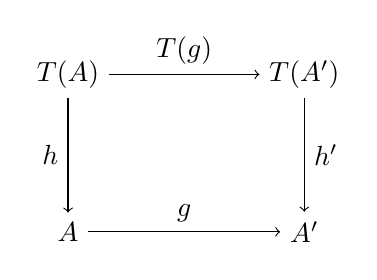
\begin{tikzpicture}
    \node (A) {$T(A)$};
    \node (B) [node distance=3cm, right of=A] { $T(A')$};
    \node (C) [node distance=2cm, below of=A]{$A$};
    \node (D) [node distance=3cm, right of=C] {$A'$};
    \draw[->] (A) to node [above,midway] {$T(g)$} (B);
    \draw[->] (C) to node [above,midway]{$g$} (D);
     \draw[->] (A) to node [left,midway] {$h$} (C);
    \draw[->] (B) to node [right,midway]{$h'$} (D);
  \end{tikzpicture}
  \]
  Recall from Remark~\ref{rem:pos-mod-alg} that a \emphind{positive modal $\Box$-algebra} is a pair $(A,\Box)$ where $A$ is a distributive lattice and $\Box$ is a unary operation on $A$ which preserves finite meets. %
  Write $T_\Box$ for the composite functor $\DL \stackrel{U}{\to} \cat{SL} \stackrel{F_\Box}{\to} \DL$. Show that the category of $T_\Box$-algebras is isomorphic to the category of positive modal $\Box$-algebras.
  \end{enumerate}
  \end{exercise}
  
  
  \begin{exercise}\label{ex:upperviet-1}
  Let $M$ be a distributive lattice. This exercise guides you through a computation of the dual space of the lattice $F_{\Box}(M)$ defined in Example~\ref{exa:modal-alg-functor}, also see Exercise~\ref{ex:boxfunctor} above and Exercise~\ref{exe:compatible-to-vietoris} in Chapter~\ref{ch:methods}.
  \begin{enumerate}
  \item Prove that the poset of prime filters of $F_\Box(M)$, under reverse inclusion, is order-isomorphic to the poset of filters of $M$, under reverse inclusion.
  \item Prove that the order-isomorphism from the previous item sends, for each $\Box a \in \Box M$, the clopen down-set $\widehat{\Box a}$ to 
  \[
  \widetilde{a} = \{F\in\Filt(M)\mid a\in F\}\ \text{ for } a\in M.
  \]

  Now denote by $X$ the Priestley dual space of $M$, so that $M$ is isomorphic to the clopen down-sets of $X$ via the isomorphism $\widehat{(-)}$. 

  \item 
  Show that the topological space $(\Filt(M),\gen{\widetilde{a}\mid a\in M})$ is homeomorphic to the \emphind{upper Vietoris space} $(\mathcal{V}(X),\tau)$, where $\mathcal{V}(X)$ is the set of closed down-sets of $X$, and $\tau$ is the topology generated by the basis consisting of the sets
  \[
  \Box a=\{K\in\mathcal{V}(X)\mid K\subseteq \widehat{a}\},\ \text{ for } a\in M.
  \]
   \hint{The functions $k:\Filt(M)\to\mathcal{V}(X), F\mapsto\bigcap\{\widehat{a}\mid a\in F\}$ and $f:\mathcal{V}(X)\to \Filt(M), K\mapsto\{a\mid K\subseteq\widehat{a}\}$ are inverse maps witnessing the homeomorphism.}
\item Prove that $\tau^\partial$, the co-compact dual topology of $\tau$, is generated by the basis consisting of finite unions of sets of the form $(\Box a)^c$, for $a \in M$.
\item Conclude that the Priestley dual space of $F_\Box(M)$ is order-homeomorphic to $(\mathcal{V}(X), \tau^p, \leq)$, where $\tau^p$ is the patch topology $\tau \vee \tau^\partial$, and $\leq$ is the \emph{inclusion} order on closed down-sets.
\item Explain how the result from the preceding item, together with Theorem~\ref{thm:unaryboxduality}, gives an alternative proof of the main result of Exercise~\ref{exe:compatible-to-vietoris}, namely that upward compatible relations $R \subseteq X \times Y$ are in bijection with continuous order-preserving functions $f \colon X \to \mathcal{V}(Y)$.
  \end{enumerate}
  \end{exercise}












\theendnotes
\setcounter{endnote}{0}

